%instiki:category: FisicaSubatomica

\chapter{Fermiones}
\label{cha:fermiones}
%instiki:
%instiki:***
%instiki:
%instiki:[[NotasFS|Tabla de Contenidos]]
%instiki:
%instiki:***
%instiki:
%instiki:* [Ecuaci\'on de Dirac](#ecuacion-de-dirac)
%instiki:
%instiki:* [Electrodin\'amica Cu\'antica](#electr-cuant)
%instiki:
%instiki:* [Cromodin\'amica Cu\'antica](#inter-fuert)
%instiki:
%instiki:* [Soluci\'on de part\'\i cula libre](#solucion-de-parti)
%instiki:
%instiki:***
%instiki:



\section{Fermiones quirales de cuatro componentes}
\label{sec:ferm-quir-de}

Sea
\begin{align}
  P_L\equiv&\frac{1-\gamma_5}{2}\nonumber\\
  P_R\equiv&\frac{1+\gamma_5}{2}\,.
\end{align}
Además
\begin{align}
  \psi_L\equiv P_L\psi\nonumber\\
  \psi_R\equiv P_R\psi\,.
\end{align}
Entonces
\begin{align}
  \psi=\psi_L+\psi_R\,.
\end{align}

Las matrices $P_{L,R}$ tienen las propiedades
\begin{align}
  P_L+P_R&=1 & P_{L,R}^2&=P_{L,R}P_{L,R}=P_{L,R}\nonumber\\
  P_L P_R&=0& P_{L,R}^\dagger&=P_{L,R}\,.
\end{align}
Usando la ec.~(\ref{eq:218qft})
\begin{align}
  P_{L,R}\gamma^\mu=\frac{1\mp\gamma_5}{2}\gamma^\mu=\gamma^\mu\frac{1\pm\gamma_5}{2}=\gamma^\mu P_{R,L}
\end{align}
Para escribir el Lagrangiano en término de los nuevos $\psi_{L,R}$ debemos tener en cuenta que
\begin{align}
  \overline{\psi_{L,R}}=(P_{L,R}\psi)^\dagger\gamma^0=\psi^\dagger P_{L,R}\gamma^0=\psi^\dagger\gamma^0P_{R,L}=\overline{\psi}P_{R,L}
\end{align}
\begin{align}
  \label{eq:221qft}
  \mathcal{L}=&i\overline{\psi}\gamma^\mu\partial_\mu\psi-m\overline{\psi}\psi\nonumber\\
  =&i\overline{\psi}(P_L+P_R)\gamma^\mu\partial_\mu\psi-m\overline{\psi}(P_L+P_R)\psi\nonumber\\
  =&i\overline{\psi}P_L\gamma^\mu\partial_\mu\psi+i\overline{\psi}P_R\gamma^\mu\partial_\mu\psi-m\overline{\psi}P_L\psi-m\overline{\psi}P_R\psi\nonumber\\
  =&i\overline{\psi}P_L P_L\gamma^\mu\partial_\mu\psi+i\overline{\psi}P_R P_R\gamma^\mu\partial_\mu\psi-m\overline{\psi}P_L P_L\psi-m\overline{\psi}P_R P_R\psi\nonumber\\
  =&i\overline{\psi}P_L\gamma^\mu\partial_\mu P_R\psi+i\overline{\psi}P_R\gamma^\mu\partial_\mu P_L\psi-m\overline{\psi}P_L P_L\psi-m\overline{\psi}P_R P_R\psi\nonumber\\
  =&i\overline{\psi_R}\gamma^\mu\partial_\mu\psi_R+i\overline{\psi_L}\gamma^\mu\partial_\mu\psi_L-m(\overline{\psi_R}\psi_L+\overline{\psi_L}\psi_R)\,.
\end{align}
En términos de espinores izquierdos y derechos de cuatro componentes la transformación de paridad 
\begin{align}
  \label{eq:220qft}
  t&\to t&\mathbf{x}&\to -\mathbf{x}&\psi_L(t,\mathbf{x})\to&\psi_R(t,-\mathbf{x}),& \psi_R(t,\mathbf{x})&\to\psi_L(t,-\mathbf{x})\nonumber\\
  \partial_0&\to \partial_0&\boldsymbol{\nabla}&\to -\boldsymbol{\nabla}&\psi_L(t,\mathbf{x})\to&\psi_R(t,-\mathbf{x}),& \psi_R(t,\mathbf{x})&\to\psi_L(t,-\mathbf{x})\,.
\end{align}
Además $\mathbf{L}=\mathbf{r}\times \mathbf{p}\to(-\mathbf{r})\times (-\mathbf{p})=\mathbf{L}$, y como $\gamma^\mu$ esta asociado al momento angular intrínsico, entonces también $\gamma^\mu\to\gamma^\mu$


Entonces la transformación de paridad da lugar a (sin tener en cuenta el cambio de argumento en los campos que desaparece en la integral de la Acción)
\begin{align}
  \overline{\psi_R}\gamma^\mu\partial_\mu\psi_R=\overline{\psi_R}\gamma^0\partial_0\psi_R+\overline{\psi_R}\boldsymbol{\gamma}\cdot\boldsymbol{\nabla}\psi_R 
\to&\overline{\psi_L}\gamma^0\partial_0\psi_L-\overline{\psi_L}\boldsymbol{\gamma}\cdot\boldsymbol{\nabla}\psi_L\nonumber\\
=&\overline{\psi_L}\gamma^0\partial_0\psi_L+\overline{\psi_L}\boldsymbol{\gamma}^\dagger\cdot\boldsymbol{\nabla}\psi_L\nonumber\\
=&\overline{\psi_L}\gamma^0\gamma^0\gamma^0\partial_0\psi_L+\overline{\psi_L}\gamma^0\boldsymbol{\gamma}\gamma^0\cdot\boldsymbol{\nabla}\psi_L\nonumber\\
=&\overline{\psi_L}\tilde\gamma^0\partial_0\psi_L+\overline{\psi_L}\tilde{\boldsymbol{\gamma}}\cdot\boldsymbol{\nabla}\psi_L\nonumber\\
=&\overline{\psi_L}\tilde\gamma^\mu\partial_\mu\psi_L\,.
\end{align}
Entonces
\begin{align}
   \mathcal{L}\to\mathcal{L}'=&i\overline{\psi_R}\tilde\gamma^\mu\partial_\mu\psi_R+i\overline{\psi_L}\tilde\gamma^\mu\partial_\mu\psi_L-m(\overline{\psi_R}\psi_L+\overline{\psi_L}\psi_R)\,,
\end{align}
donde $\tilde\gamma^\mu=U\gamma^\mu U^\dagger$, con $U=\gamma^0$. Como las dos representaciones dan lugar a la misma física, podemos decir que la Acción en términos de espinores $L,R$ de cuatro componentes es invariante bajo la transformación de paridad.

La existencia de ambos espinores $\psi_{L,R}$ garantizan que el Lagrangiano de Dirac es invariante bajo la transformación de paridad. 

La corriente de la electrodinámica cuántica en ec.~\eqref{eq:222qft} (o la de la cromodinámica cuántica, ec.~\eqref{eq:223qft}) conservan paridad ya que, siguiendo los mismos pasos que en la ec.~\eqref{eq:221qft}
\begin{align}
  \label{eq:224qft}
  \overline{\psi}\gamma^\mu\psi=\overline{\psi_L}\gamma^\mu\psi_L+\overline{\psi_R}\gamma^\mu\psi_R\to\overline{\psi_L}\tilde{\gamma}^\mu\psi_L+\overline{\psi_R}\tilde{\gamma}^\mu\psi_R\,.
\end{align}
Si para alguna partícula, como es el caso del neutrino, no existe la componente derecha, entonces la correspondiente interacción vectorial viola paridad y no puede tener ni interacciones electromagnéticas ni fuertes, es decir, no se acopla con el fotón o los gluones. Además dicha partícula no puede tener masa de Dirac. En el caso del neutrino esto se entiende pues al no tener carga eléctrica sólo requiere dos grados de libertad independientes.

De otro lado, si una determinada interacción, como es el caso de la interacción débil, solo participa la componente izquierda de la ec.~\eqref{eq:224qft}, está corresponde a una interacción del tipo
\begin{align}
  \overline{\psi}_L\gamma^\mu\psi_L&=\overline{\psi}P_R\gamma^\mu P_L\psi=\overline{\psi}\gamma^\mu P_L\psi\nonumber\\
  &=\overline{\psi}\gamma^\mu\left(\frac{1-\gamma_5}{2}\right)\psi\nonumber\\
  &=\tfrac{1}{2}\overline{\psi}\left(\gamma^\mu-\gamma^\mu\gamma_5\right)\psi\,,
\end{align}
que de acuerdo a la asignación en la Tabla corresponde a una corriente V--A. 

\subsection{Fermiones de Weyl}
\label{sec:fermiones-de-weyl}
%Weyl because $\psi^\dagger$ instead $\bar \psi$
Sea $\psi$ un campo que satisface una ecuaci\'on covariante de segundo orden. La parte cin\'etica del Lagrangiano sin t\'erminos de masa y sin t\'erminos de interacci\'on debe tener la forma 
\begin{equation}
\label{eq:98}
  \mathcal{L}=\frac{i}{2}\psi^\dagger a^\mu\partial_\mu\psi-\frac{i}{2}\partial_\mu\psi^\dagger {a^\mu}^\dagger\psi-m\psi^\dagger b\psi
\end{equation}
La Acci\'on debe ser real, de modo que el Lagrangiano tambi\'en. En efecto
\begin{align*}
  \mathcal{L}^\dagger&=\left(\frac{i}{2}\psi^\dagger a^\mu\partial_\mu\psi-\frac{i}{2}\partial_\mu\psi^\dagger {a^\mu}^\dagger\psi\right)^\dagger-m\psi^\dagger b^\dagger \psi\\
  &=\left(-\frac{i}{2}\partial^\mu\psi^\dagger a_\mu^\dagger \psi+\frac{i}{2}\psi^\dagger {a^\mu} \partial_\mu\psi\right)-m\psi^\dagger b^\dagger \psi\\
  &=\mathcal{L} \qquad \text{si }b^\dagger = b\,.
\end{align*}
Como al aplicar las ecuaciones de Euler-Lagrange a este Lagrangiano debemos obtener la ecuaci\'on de Scrh\"odinger
\begin{align}
i\frac{\partial}{\partial t}\psi=\widehat{H}\psi
\end{align}
con $\widehat{H}$ una funci\'on por determinar del operador $\hat{\mathbf{p}}$, entonces
\begin{align}
  a_\mu^\dagger=a_\mu
\end{align}

El Lagrangiano en ec.~(\ref{eq:98}) puede reescribirse como
\begin{align}
  \label{eq:197}
  \mathcal{L}&=\frac{i}{2}\psi^\dagger a^\mu\partial_\mu\psi-\frac{i}{2}\partial_\mu\left(\psi^\dagger a^\mu\psi\right)+\frac{i}{2}\psi^\dagger a^\mu\partial_\mu\psi-m\psi^\dagger b\psi\nonumber\\
  &=i \psi^\dagger a^\mu\partial_\mu\psi-\frac{i}{2}\partial_\mu\left(\psi^\dagger a^\mu\psi\right)-m\psi^\dagger b\psi\nonumber\\
  \mathcal{L}&=i \psi^\dagger a^\mu\partial_\mu\psi-m\psi^\dagger b\psi
\end{align}

Ahora utilizaremos el m\'etodo desarrollado en cap\'\i tulos anteriores para analizar el Lagrangiano. Calcularemos las ecuaciones de Euler-Lagrange, la corriente conservada y el tensor de momento-energ\'\i a.


\section{Soluciones a la ecuaci\'on de Dirac}
\label{sec:soluc-la-ecuac}

\subsection{Lagrangiano de Weyl}
\label{sec:lagrangiano-de-weyl}


En la ec.~\eqref{eq:118}, obtuvimos el Hamiltoniano en ec.~\eqref{eq:103}
\begin{equation}
  \hat{H}= \gamma_0(\boldsymbol{\gamma}\cdot\mathbf{p}+m)=\boldsymbol{\alpha}\cdot\mathbf{p}+\beta m\,.
\end{equation}
Una escogencia particular de las cuatro matrices $\gamma^\mu$, conocida como la representaci\'on de Weyl, o representaci\'on quiral, puede escribirse en t\'erminos de la matrices de Pauli. Escritas en bloques $2\times2$, tenemos
\begin{equation}
  \gamma^0=
  \begin{pmatrix}
    0&\sigma_0\\
    \sigma_0&0
  \end{pmatrix}\qquad
  \gamma_i=\begin{pmatrix}
    0&\sigma_i\\
    -\sigma_i&0
  \end{pmatrix}.
\end{equation}
Con $\sigma^0=1$. Con la matriz de tranformaci\'on
\begin{equation}
  U=\frac{1}{\sqrt{2}}
  \begin{pmatrix}
    1&1\\
    -1&1    
  \end{pmatrix}
\end{equation}
podemos obtener la representaci\'on de Dirac, tal que $U$ diagonaliza $\gamma^0$,
\begin{equation}
  \gamma^0=
  \begin{pmatrix}
    \sigma^0&0\\
    0&-\sigma^0
  \end{pmatrix}\qquad
  \gamma_i=\begin{pmatrix}
    0&\sigma_i\\
    -\sigma_i&0
  \end{pmatrix}.
\end{equation}
En adelante trabajaremos en la representaci\'on de Weyl que en forma compacta es
\begin{equation}
  \gamma^\mu=\begin{pmatrix}
    0&\sigma^\mu\\
    \bar{\sigma}^\mu & 0
  \end{pmatrix}
\end{equation}
donde
\begin{align}
  \sigma^\mu&=(\sigma^0,\sigma^1,\sigma^2,\sigma^3)\nonumber\\
  \bar{\sigma}^\mu&=(\sigma^0,-\sigma^1,-\sigma^2,-\sigma^3)\nonumber\\
\end{align}
Hemos escrito las matrices de Dirac en bloques $2\times2$, y es natural escribir similarmente las cuatro componentes del campo de Dirac como un par de campos de dos componentes
\begin{align}
  \psi=  \begin{pmatrix}
    \psi_L\\
    \psi_R    
  \end{pmatrix}=\begin{pmatrix}
    \psi_L\\
    0   
  \end{pmatrix}+\begin{pmatrix}
    0\\
    \psi_R    
  \end{pmatrix}
\end{align}
Donde $\psi_{L,R}$ son espinores de Weyl de dos componentes. En la representaci\'on de Weyl el Lagrangiano se puede escribir como
\begin{align}
\label{eq:200}
  \mathcal{L}=&i\bar{\psi}\gamma^\mu\partial_\mu\psi-m\bar{\psi}\psi\nonumber\\
  =&i\psi^\dagger \gamma^0\gamma^\mu\partial_\mu\psi-m\psi^\dagger \gamma^0 \psi\nonumber\\
  =&i\psi^\dagger  \begin{pmatrix}
    0 & 1\\
    1&0
  \end{pmatrix}
  \begin{pmatrix}
    0 &\sigma^\mu \\
    \bar{\sigma}^\mu&0
  \end{pmatrix}\partial_\mu\psi-m\psi^\dagger
  \begin{pmatrix}
    0 & 1\\
    1&0
  \end{pmatrix}\psi\nonumber\\
=&i\begin{pmatrix}
 \psi_L^\dagger & \psi_R^\dagger
\end{pmatrix}
 \begin{pmatrix}
   \bar{\sigma}^\mu &0\\
   0&\sigma^\mu
 \end{pmatrix} \begin{pmatrix}
   \partial_\mu\psi_L\\
   \partial_\mu\psi_R
 \end{pmatrix}-m
 \begin{pmatrix}
   \psi_L^\dagger&\psi_R^\dagger
 \end{pmatrix}
 \begin{pmatrix}
   0&1\\
   1&0
 \end{pmatrix}
 \begin{pmatrix}
   \psi_L\\ \psi_R
 \end{pmatrix}\nonumber\\
 =& i\psi_L^\dagger \bar{\sigma}^\mu\partial_\mu\psi_L+i\psi_R^\dagger \sigma^\mu\partial_\mu\psi_R
  -m(\psi_L^\dagger \psi_R+\psi_R^\dagger \psi_L)
\end{align}

\subsection{Ecuaciones de Weyl}
\label{sec:ecuaciones-de-weyl}
Las ecuaciones de Euler-Lagrango para el Lagrangiano en ec.\eqref{eq:200}, dan como resultado
\begin{align}
  i\bar{\sigma}^\mu\partial_\mu\psi_L -m\psi_R &=0\nonumber\\
  i{\sigma}^\mu\partial_\mu\psi_R -m\psi_L &=0
\end{align}
Expandiendo
\begin{align}
  \label{eq:209}
   i{\sigma}^0\partial_0\psi_L-i{\sigma}^i\partial_i\psi_L -m\psi_R &=0\nonumber\\
   i{\sigma}^0\partial_0\psi_R+i{\sigma}^i\partial_i\psi_R -m\psi_L &=0
\end{align}
que pueden escribirse como
\begin{align}
  \label{eq:207}
   i\partial_0\psi_L-i\boldsymbol{\sigma}\cdot\boldsymbol{\nabla}\psi_L -m\psi_R &=0\nonumber\\
   i\partial_0\psi_R+i\boldsymbol{\sigma}\cdot\boldsymbol{\nabla}\psi_R -m\psi_L &=0
\end{align}
Para el Lagrangiano invariante gauge local $U(1)$ en ec.\eqref{eq:201}, tendr\'\i amos
\begin{align}
  i\bar{\sigma}^\mu\mathcal{D}_\mu\psi_L -m\psi_R &=0\nonumber\\
  i{\sigma}^\mu\mathcal{D}_\mu\psi_R -m\psi_L &=0
\end{align}
Expandiendo, para $\mathcal{D}^\mu$ dado en la ec.\eqref{eq:202}, con $q=-e$
\begin{equation}
  \mathcal{D}_\mu=\partial_\mu+i q A_\mu
\end{equation}
Tenemos
\begin{align}
     i(\partial_0+i q A_0)\psi_L-i{\sigma}^i(\partial_i+i q A_i)\psi_L -m\psi_R &=0\nonumber\\
   i(\partial_0+i q A_0)\psi_R+i{\sigma}^i(\partial_i+i q A_i)\psi_R -m\psi_L &=0
\end{align}
de donde
\begin{align}
\label{eq:203}
     (i\partial_0- q A_0)\psi_L-{\sigma}^i(i\partial_i-q A_i)\psi_L -m\psi_R &=0\nonumber\\
   (i\partial_0-q A_0)\psi_R+{\sigma}^i(i\partial_i-q A_i)\psi_R -m\psi_L &=0
\end{align}
\section{Esp\'\i n}
\label{sec:espin}
El momento angular est\'a descrito por el \'algebra
\begin{equation}
  [\hat L_i,\hat L_j]=i\epsilon_{ijk}\hat L_k
\end{equation}
Si dos operadores no conmutan no es posible conocer sus autovalores simult\'aneamente. Sin embargo
\begin{equation}
  [\hat L_i,\hat{L}^2]=0
\end{equation}
y por convenci\'on podemos escoger $\langle\hat L_z\rangle$ y $\hat{L}^2$ como los dos observables de momento \'angular. 

Las matrices de Pauli forman una representaci\'on del \'algebra de momento angular
\begin{equation}
  [\hat S_i,\hat S_j]=i\epsilon_{ijk}\hat S_k
\end{equation}
donde el \emph{operador de esp\'\i n} se define como
\begin{equation}
  \hat S_i=\frac{\sigma_i}{2}
\end{equation}
Los autovalores del operador de esp\'\i n son entonces
\begin{equation}
  \hat S_z
  \begin{pmatrix}
    a\\
    b
  \end{pmatrix}=\lambda
  \begin{pmatrix}
    a\\
    b
  \end{pmatrix}
\end{equation}
que corresponde a autovalores $\lambda=\pm1/2$ con autovectores 
\begin{equation}
  |\uparrow\rangle=\begin{pmatrix}
    1\\
    0
  \end{pmatrix}\qquad
  |\downarrow\rangle=\begin{pmatrix}
    0\\
    1
  \end{pmatrix}
\end{equation}
que son autoestados de esp\'\i n up y esp\'\i n down respectivamente. Una funci\'on de onda de esp\'\i n ha de poder expandir en t\'erminos de estos autoestados
\begin{equation}
  |\psi\rangle=c_1|\uparrow\rangle+c_2|\downarrow\rangle
\end{equation}
donde $|c_1|^2$ y $|c_2|^2$ corresponden a las probabilidades de encontrar el estado con esp\'\i n up o esp\'\i n down respectivamente. Adem\'as
\begin{equation}
  |c_1|^2+|c_2|^2=1
\end{equation}
y $\psi$ es un espinor. La ecuaci\'on de Scr\"odinger para un espinor es, por ejemplo
\begin{align}
  i\frac{\partial\psi_R}{\partial t}=\widehat{H}\psi_R
\end{align}
donde
\begin{equation}
  \psi_R=
  \begin{pmatrix}
    \psi_1\\
    \psi_2
  \end{pmatrix}
\end{equation}
con $\psi_i$ las funciones de onda convencionales. Dicha ecuaci\'on debe ser invariante bajo rotaciones en el espacio de esp\'\i n
\begin{equation}
  \psi_R\to\psi'_R=\exp(i\frac{\sigma^i}{2}\theta_i)\psi_R\,.
\end{equation}
Esta es justo las ecuaciones que aparecen cuando se hace $m=0$ en la ec.\eqref{eq:207}. Para $\psi_R$
\begin{equation}
  \widehat{H}=i\boldsymbol{\sigma}\cdot\boldsymbol{\nabla}=-\boldsymbol{\sigma}\cdot\mathbf{p}
\end{equation}
con
\begin{align}
\label{eq:208}
\mathcal{L}&= i\psi_R^\dagger {\sigma}^\mu\partial_\mu\psi_R  \nonumber\\
&=i\psi_R^\dagger \partial_0\psi_R+i\psi_R^\dagger {\sigma}^i\partial_i\psi_R\nonumber\\
&=i\psi_R^\dagger \partial_0\psi_R-i\psi_R^\dagger\boldsymbol{\sigma}\cdot\mathbf{p} \psi_R
\end{align}
Como el Lagrangiano debe ser escalar entonces $\psi_R^\dagger\boldsymbol{\sigma} \psi_R$ debe ser un vector en el espacio de esp\'\i n. En efecto, escogiendo los coeficientes como
\begin{align}
  c_1&=e^{-i \phi/2}\cos(\theta/2)\nonumber\\
  c_2&=e^{i \phi/2}\sin(\theta/2)
\end{align}
entonces
\begin{equation}
  |c_1|^2+|c_2|^2=c_1 c_1^*+c_2 c_2^*=\cos^2(\theta/2)+\sin^2(\theta/2)=1\,.
\end{equation}
Para
\begin{align}
  \psi_R=e^{-i p\cdot x}(c_1|\uparrow\rangle+c_2|\downarrow\rangle)&=e^{-i p\cdot x}\left[c_1\begin{pmatrix}
    1\\
    0
  \end{pmatrix}+c_2
  \begin{pmatrix}
    0\\
    1
  \end{pmatrix}\right]=
  e^{-i p\cdot x}\begin{pmatrix}
    c_1\\
    c_2
  \end{pmatrix}\,\nonumber\\
  &=e^{-i p\cdot x}
  \begin{pmatrix}
  e^{-i \phi/2}\cos(\theta/2)\\
  e^{i \phi/2}\sin(\theta/2)
  \end{pmatrix}=e^{-i p\cdot x}|+\rangle
\end{align}
donde
\begin{equation}
|+\rangle=  \begin{pmatrix}
  e^{-i \phi/2}\cos(\theta/2)\\
  e^{i \phi/2}\sin(\theta/2)
  \end{pmatrix}\,.
\end{equation}
Tenemos
\begin{align}
  \psi^\dagger_R \sigma_1 \psi_R=&
  \begin{pmatrix}
   c_1^\dagger & c_2^\dagger 
  \end{pmatrix}
  \begin{pmatrix}
    0 & 1\\
    1&0
  \end{pmatrix}
  \begin{pmatrix}
    c_1\\
    c_2
  \end{pmatrix}\nonumber\\
  =&  \begin{pmatrix}
    c_2^\dagger & c_1^\dagger
  \end{pmatrix}
  \begin{pmatrix}
    c_1\\
    c_2
  \end{pmatrix}\nonumber\\
  =&  c_2^\dagger c_1 + c_1^\dagger c_2\nonumber\\
  =&  \sin(\theta/2)\cos(\theta/2)e^{-i\phi}+\cos(\theta/2)\sin(\theta/2)e^{i\phi}\nonumber\\
  =&  (e^{-i\phi}+e^{i\phi})\cos(\theta/2)\sin(\theta/2)\nonumber\\
  =&  (2\cos\phi)\frac{1}{2}\sin\theta\nonumber\\
  =&  \cos\phi\sin\theta
\end{align}
Similarmente
\begin{align}
  \psi^\dagger_R \sigma_2\psi_R&=\sin\phi\sin\theta\nonumber\\
  \psi^\dagger_R \sigma_3\psi_R&=\cos\theta
\end{align}
Por consiguiente $\psi^\dagger \sigma_i\psi$ son las componentes de un vector unitario $\psi^\dagger \boldsymbol{\sigma}\psi$ con \'angulo polar $\theta$ y \'angulo azimutal $\phi$. Posibles escalares se pueden construir con otros vectores disponibles, por ejemplo $\mathbf{p}$, como en la ec.~\eqref{eq:208}.
\begin{align}
  \boldsymbol{\sigma}\cdot\hat{\mathbf{p}}=&\sigma^i \frac{p^i}{|\mathbf{p}|}\nonumber\\
  =&\sigma^1\cos\phi\sin\theta+\sigma^2\sin\phi\sin\theta+\sigma^3\cos\theta\nonumber\\
  =&\begin{pmatrix}
    \cos\theta&\sin\theta(\cos\phi-i\sin\phi)\\
    \sin\theta(\cos\phi-i\sin\phi)&-\cos\theta
  \end{pmatrix}\nonumber\\
  =&\begin{pmatrix}
    \cos\theta&e^{-i\phi}\sin\theta\\
    e^{i\phi}\sin\theta&-\cos\theta
  \end{pmatrix}
\end{align}
\begin{align}
\boldsymbol{\sigma}\cdot\hat{\mathbf{p}}|+\rangle=&\begin{pmatrix}
    \cos\theta&e^{-i\phi}\sin\theta\\
    e^{i\phi}\sin\theta&-\cos\theta
  \end{pmatrix}\begin{pmatrix}
  e^{-i \phi/2}\cos(\theta/2)\\
  e^{i \phi/2}\sin(\theta/2)
  \end{pmatrix}\nonumber\\
  =&e^{-i\phi/2}\begin{pmatrix}
    \cos\theta&e^{-i\phi}\sin\theta\\
    e^{i\phi}\sin\theta&-\cos\theta
  \end{pmatrix}\begin{pmatrix}
  \cos(\theta/2)\\
  e^{i \phi}\sin(\theta/2)
  \end{pmatrix}\nonumber\\
  =&e^{-i\phi/2}
  \begin{pmatrix}
    \cos\theta\cos(\theta/2)+\sin\theta\sin(\theta/2)\\
    e^{i\phi}[\sin\theta\cos(\theta/2)- \cos\theta\sin(\theta/2)]
  \end{pmatrix}\nonumber\\
  =&e^{-i\phi/2}
  \begin{pmatrix}
    \cos(\theta-\theta/2)\\
    e^{i\phi}\sin(\theta-\theta/2)
  \end{pmatrix}\nonumber\\
  =&e^{-i\phi/2}
  \begin{pmatrix}
    \cos(\theta/2)\\
    e^{i\phi}\sin(\theta/2)
  \end{pmatrix}\nonumber\\
  =&+|+\rangle
\end{align}
(El gorro en este caso, significa vector unitario). Decimos entonces que
\begin{align}
\label{eq:214}
\boldsymbol{\sigma}\cdot\hat{\mathbf{p}}\psi_R=+e^{-i p\cdot x}|+\rangle=+\psi_R
\end{align}
es un estado de helicidad positiva o derecha. Como $\boldsymbol{\sigma}\cdot\mathbf{p}$ denota la proyecci\'on de esp\'\i n sobre la direcci\'on de moviento, para la helicidad derecha, dicha proyecci\'on es positiva.


Si definimos ademas
\begin{equation}
  \psi_L=e^{-i p\cdot x}|-\rangle
\end{equation}
donde
\begin{equation}
|-\rangle=  \begin{pmatrix}
  -e^{-i \phi/2}\sin(\theta/2)\\ 
  e^{i \phi/2}\cos(\theta/2)
  \end{pmatrix}\,,
\end{equation}
entonces
\begin{align}
  \psi^\dagger\boldsymbol{\sigma}\cdot\hat{\mathbf{p}}\psi=-(\cos\phi\sin\theta,\sin\phi\sin\phi,\cos\theta)
\end{align}
y
\begin{equation}
  \label{eq:215}
  \boldsymbol{\sigma}\cdot\hat{\mathbf{p}}\psi_L=-e^{-i p\cdot x}|-\rangle=-\psi_L
\end{equation}
$\psi$ es un estado de helicidad negativa o izquierda. Adem\'as
\begin{align}
  \langle-|-\rangle=\langle+|+\rangle=1\qquad \langle+|-\rangle=\langle-|+\rangle=0
\end{align}
donde $\langle-|=|-\rangle^\dagger$, etc.
%\left(\right)
\section{Soluci\'on de part\'\i cula libre}
\label{sec:solucion-de-parti}
Consideraremos incialmente dos casos $m^2\gg\mathbf{p}^2$ y $m^2\ll\mathbf{p}^2$.

De la ecuaci\'on relativista
\begin{equation}
  \label{eq:213}
  E^2=\mathbf{p}^2+m^2\,,
\end{equation}
tenemos que para elcaso no relativista $m^2\gg\mathbf{p}^2$, podemos tomar $\mathbf{p}=0$, de modo que
\begin{equation}
  E^2=m^2\Rightarrow E=\pm m
\end{equation}
La aparici\'on de soluciones de Energ\'\i a negativa. . .

A $\mathbf{p}=0$ proponemos las soluciones de energ\'\i a positiva $E=+m$
\begin{align}
  \label{eq:210}
  \psi_L&=u_L e^{-i E t}=\psi_L=u_L e^{-i m t} & \psi_R&=u_R e^{-i E t}=u_R e^{-i m t}
\end{align}

En este caso las ecs.~\eqref{eq:207} se reducen a
\begin{align}
  i\partial_0\psi_L -m\psi_R &=0\nonumber\\
  i\partial_0\psi_R -m\psi_L &=0
\end{align}
de modo que para que \eqref{eq:210} sea soluci\'on, se debe satisfacer que 
\begin{equation}
  u_L=u_R=u
\end{equation}
con
\begin{align}
  u=  \begin{pmatrix}
    u_1\\
    u_2    
  \end{pmatrix}=|+\rangle\,.
\end{align}
El espinor completo es
\begin{align}
  \psi=\begin{pmatrix}
    \psi_L\\
    \psi_R
  \end{pmatrix}=e^{-i m t}\begin{pmatrix}
    |+\rangle\\
    |+\rangle
  \end{pmatrix}
\end{align}
Con norma
\begin{align}
  \bar{\psi}\psi=\psi^\dagger\gamma^0\gamma^0\psi=\psi^\dagger\psi=|+\rangle^\dagger|+\rangle+|+\rangle^\dagger|+\rangle=1
\end{align}
Para el caso relativista $m^2\ll\mathbf{p}^2$, podemos hacer $m=0$ y las ecuaciones \eqref{eq:207} se desacoplan
\begin{align}
  \label{eq:211}
   i\partial_0\psi_L-i\boldsymbol{\sigma}\cdot\boldsymbol{\nabla}\psi_L &=0\nonumber\\
   i\partial_0\psi_R+i\boldsymbol{\sigma}\cdot\boldsymbol{\nabla}\psi_R&=0
\end{align}
Proponemos como soluciones de energ\'\i a positiva
\begin{align}
  \label{eq:212}
    \psi_L&=u_L e^{-i p\cdot x}=\psi_L=u_L e^{i(\mathbf{p}\cdot \mathbf{x}-E t)} & \psi_R&=u_R e^{-i p\cdot x}=u_R e^{i(\mathbf{p}\cdot \mathbf{x}-E t)}
\end{align}
reemplazando en las ecs.~\eqref{eq:211} tenemos
\begin{align}
  \label{eq:217}
     E\psi_L+\boldsymbol{\sigma}\cdot\mathbf{p}\psi_L &=0\nonumber\\
   E\psi_R-\boldsymbol{\sigma}\cdot\mathbf{p}\psi_R&=0
\end{align}
De modo que para que las ecs.~\eqref{eq:212} sean soluci\'on se debe satisfacer que
\begin{align}
     \boldsymbol{\sigma}\cdot\frac{\mathbf{p}}{E}\psi_L &=-\psi_L\nonumber\\
   \boldsymbol{\sigma}\cdot\frac{\mathbf{p}}{E}\psi_R&=\psi_R
\end{align}
pero de la ec.~\eqref{eq:213}, tenemos que para $m=0$, $E=|\mathbf{p}|$, y $\mathbf{p}/E=\mathbf{p}/|\mathbf{p}|=\hat{\mathbf{p}}$. Entonces
\begin{align}
  \boldsymbol{\sigma}\cdot\hat{\mathbf{p}}\psi_L &=-\psi_L\nonumber\\
  \boldsymbol{\sigma}\cdot\hat{\mathbf{p}}\psi_R&=\psi_R
\end{align}
Comparando con las ecuaciones \eqref{eq:214} y \eqref{eq:215} vemos que para las soluciones de energ\'\i a positiva $\psi_{R,L}$ corresponden en efecto a estado de helicidad derecha e izquierda respectivamente. Explicitamente
\begin{equation}
  \boldsymbol{\sigma}\cdot\hat{\mathbf{p}}\psi_L=e^{-i p\cdot x}\boldsymbol{\sigma}\cdot\hat{\mathbf{p}}|-\rangle=-e^{-i p\cdot x}|-\rangle=-\psi_L
\end{equation}
El espinor de cuatro componentes para la soluci\'on de energ\'\i a positiva es
\begin{equation}
  \psi=\begin{pmatrix}
    \psi_L\\
    \psi_R
  \end{pmatrix}=e^{-i p\cdot x}\begin{pmatrix}
    |-\rangle\\
    |+\rangle
  \end{pmatrix}
\end{equation}

\begin{align}
  \bar{\psi}\psi=&\bar{u}{u}=\psi^\dagger \gamma^0 \psi\nonumber\\
  =&\begin{pmatrix}
    |-\rangle^\dagger & |+\rangle^\dagger
  \end{pmatrix}
  \begin{pmatrix}
    0&1\\
    1&0    
  \end{pmatrix}
  \begin{pmatrix}
    |-\rangle\\
    |+\rangle
  \end{pmatrix}\nonumber\\
  =&\begin{pmatrix}
    \langle-| & \langle+|
  \end{pmatrix}
  \begin{pmatrix}
    0&1\\
    1&0    
  \end{pmatrix}
  \begin{pmatrix}
    |-\rangle\\
    |+\rangle
  \end{pmatrix}\nonumber\\
  =&\begin{pmatrix}
    \langle+| & \langle-| 
  \end{pmatrix}
  \begin{pmatrix}
    |-\rangle\\
    |+\rangle
  \end{pmatrix}\nonumber\\
  =&\langle+|-\rangle+\langle-|+\rangle=0
\end{align}

Es convenci\'on escoger la normalizaci\'on del espinor de Dirac tal que
\begin{equation}
  \bar{u}{u}=2m
\end{equation}
que de hecho es cero cuando $m=0$.

Para las soluciones de energ\'\i a negativa tenemos

\begin{align}
    \hat{\psi}_L&=u_L e^{i(\mathbf{p}\cdot \mathbf{x}+E t)} & \hat{\psi}_R&=u_R e^{i(\mathbf{p}\cdot \mathbf{x}+E t)}
\end{align}
Para explorar las caracter\'\i sticas de esta soluci\'on podemos reemplazar en la ec.~(\ref{eq:217}) $E\to-E$, $\mathbf{p}\to\mathbf{p}$, de modo que
\begin{align}
  \boldsymbol{\sigma}\cdot\hat{\mathbf{p}}\hat{\psi}_L &=+\hat{\psi}_L\nonumber\\
  \boldsymbol{\sigma}\cdot\hat{\mathbf{p}}\hat{\psi}_R&=-\hat{\psi}_R
\end{align}
De modo que la antipart\'\i cula de una part\'\i cula de helicidad izquierda tiene helicidad derecha. Dentro de los errores experimentales actuales se puede afirmar que en la naturaleza solo se ha observado el neutrino izquierdo y su correspondiente antineutrino derecho.

Para $m\neq0$, tenemos de la ecs.~\eqref{eq:207} y \eqref{eq:212} (ver ec.~\eqref{eq:217})
\begin{align}
  E\psi_L+\boldsymbol{\sigma}\cdot\mathbf{p}\psi_L &=m\psi_R\nonumber\\
  E\psi_R-\boldsymbol{\sigma}\cdot\mathbf{p}\psi_R&=m\psi_L
\end{align}
Entonces
\begin{align}
  \label{eq:219}
  \left(\frac{E+\boldsymbol{\sigma}\cdot\mathbf{p}}{m}\right)\psi_L&=\psi_R\nonumber\\
  \left(\frac{E-\boldsymbol{\sigma}\cdot\mathbf{p}}{m}\right)\psi_R&=\psi_L\,.
\end{align}
En este caso sin embargo, la helicidad no esta bien definida y s\'olo podemos afirmar que $\psi_L$ corresponde a la soluci\'on que tiene mayor probabilidad de ser izquierda que derecha. Para calcular dicha probabilidad es necesario especificar los espinores $u_{L,R}$ (ver \cite{cottingham}, Cap\'\i tulo 6). El resultado es que la probabilidad de que $\psi_{R}$ sea derecho se obtiene de
\begin{align}
  \boldsymbol{\sigma}\cdot\mathbf{p}|\psi_{R}\rangle&=+\frac{1}{2}\left(1+\frac{v}{c}\right)|\psi_{R}\rangle\to 
  \begin{cases}
    +|\psi_{R}\rangle & v\to c\quad\text{(relativistic)}\\
    +\frac{1}{2}|\psi_{R}\rangle & v\to 0 \quad\text{(non-relativistic)}
  \end{cases}\nonumber\\
  \boldsymbol{\sigma}\cdot\mathbf{p}|\psi_{L}\rangle&=-\frac{1}{2}\left(1-\frac{v}{c}\right)|\psi_{R}\rangle
\end{align}
mientras que la probabilidad de que sea izquierdo se obtiene de
\begin{align}
\label{eq:259}
  \boldsymbol{\sigma}\cdot\mathbf{p}|\psi_{R}\rangle&=+\frac{1}{2}\left(1-\frac{v}{c}\right)|\psi_{R}\rangle\nonumber\\
  \boldsymbol{\sigma}\cdot\mathbf{p}|\psi_{L}\rangle&=-\frac{1}{2}\left(1+\frac{v}{c}\right)|\psi_{R}\rangle
\end{align}

Si en un decaimiento $\beta$ solo se emiten electrones izquierdos, el grado de polarizaci\'on del electr\'on emitido es, usando la ec.~\eqref{eq:259}
\begin{align}
   \langle \psi_R|\boldsymbol{\sigma}\cdot\mathbf{p}|\psi_R\rangle+ \langle \psi_L|\boldsymbol{\sigma}\cdot\mathbf{p}|\psi_L\rangle
=&+\frac{1}{2}\left(1-\frac{v}{c}\right)-\frac{1}{2}\left(1+\frac{v}{c}\right)=-\frac{v}{c}
\end{align}
El grafico de polarizaci\'on versus $-v/c$, \cite{cottingham} (\S9.1), debe corresponder a una l\'\i nea recta de pendiente $45^\text{o}$. Si s\'olo se emiten electrones derechos ser\'\i a
\begin{align}
  +\frac{1}{2}\left(1+\frac{v}{c}\right)-\frac{1}{2}\left(1-\frac{v}{c}\right)=\frac{v}{c}
\end{align}
Mientras que si se emiten por igual electrones derechos e izquierdos la polarizaci\'on total ser\'\i a cero.

Las soluciones en ec.~\eqref{eq:219} puden ser intercambiadas por $\psi_L\to -\psi_R$. Esto se puede ver como una transformaci\'on de paridad definida por
\begin{align}
  \mathbf{r}&\to-\mathbf{r}& t&\to t& \psi_L\leftrightarrow \psi_R\,.
\end{align}
De aqu\'\i{} el nombre de la transformaci\'on. Como $\hat{\mathbf{p}}=-i\boldsymbol{\nabla}$ y $\mathbf{L}=\mathbf{r}\times\mathbf{p}$, entonces
\begin{align}
  \mathbf{p}&\to-\mathbf{p}& \mathbf{L}\to\mathbf{L}\,,
\end{align}
Entonces es de esperarse que el momentum angular intr\'\i nseco, transforme como el momentum angular, y
\begin{align}
  \mathbf{S}&\to \mathbf{S}\Rightarrow& \boldsymbol{\sigma}\to\boldsymbol{\sigma}\,.
\end{align}
Bajo la transformaci\'on de paridad
\begin{align}
   \mathbf{p}&\to-\mathbf{p}& \boldsymbol{\sigma}&\to \boldsymbol{\sigma}& \psi_L\leftrightarrow &\psi_R\,,
\end{align}
Las ecuaciones \eqref{eq:219} quedan invariantes. Adem\'as bajo dicha transformaci\'on
\begin{align}
  \sigma^\mu\partial_\mu=\sigma^0\partial_0+\boldsymbol{\sigma}\cdot\boldsymbol{\nabla}\to \sigma^0\partial_0-\boldsymbol{\sigma}\cdot\boldsymbol{\nabla}=\bar{\sigma}^\mu\partial_\mu
\end{align}
de modo que el Lagrangiano correspondiente, dado en la ec.~\eqref{eq:200} tambi\'en es invariante bajo la transformaci\'on de paridad
\begin{align}
  \sigma^\mu\partial_\mu\to& \bar{\sigma}^\mu\partial_\mu &\psi_L\leftrightarrow &\psi_R
\end{align}



\section{L\'\i mite no relativista en presencia de un campo electromagn\'etico}
\label{sec:limite-no-relat}
En el l\'\i mitie no relativista, la ecuaci\'on de Dirac en presencia de un campo electromagn\'etico (electrodin\'amica cu\'antica en la secci\'on \ref{sec:electr-cuant}) debe contener la ecuaci\'on de Scr\"odinger en presencia de un campo electromagn\'etico.
Combinando las ecuaciones \eqref{eq:203} tenemos
\begin{align}
  \label{eq:204}
  (i\partial_0- q A_0)(\psi_L+\psi_R)-{\sigma}^i(i\partial_i-q A_i)(\psi_L-\psi_R) -m(\psi_L+\psi_R) &=0\nonumber\\
  (i\partial_0-q A_0)(\psi_L-\psi_R)-{\sigma}^i(i\partial_i-q A_i)(\psi_L+\psi_R) +m(\psi_L-\psi_R) &=0
\end{align}
Esta forma es \'util porque de la soluci\'on de part\'\i culas libre esperamos que $\psi_L-\psi_R$ sea peque\~na. 
Como antes prongamos como soluci\'on
\begin{align}
  \psi_L=&u_L e^{-i p\cdot x} & \psi_R=&u_R e^{-i p\cdot x}
\end{align}

Para solucionar este sistema de ecuaciones acopladas definimos
\begin{align}
  \label{eq:216}
  \phi=e^{i m t}(\psi_L+\psi_R)&\Rightarrow(\psi_L+\psi_R)=e^{-i m t}\phi\nonumber\\
  \chi=e^{i m t}(\psi_L-\psi_R)&\Rightarrow(\psi_L-\psi_R)=e^{-i m t}\chi
\end{align}
donde
\begin{align}
\label{eq:260}
    \phi=&e^{i m t}(\psi_L+\psi_R)=e^{i m t}e^{-i (Et-\mathbf{p}\cdot x)}(u_L+u_R)=e^{i(m-E)t}e^{i\mathbf{p}\cdot x}(u_L+u_R)\nonumber\\
    \chi=&e^{i m t}(\psi_L-\psi_R)=e^{i m t}e^{-i (Et-\mathbf{p}\cdot x)}(u_L-u_R)=e^{i(m-E)t}e^{i\mathbf{p}\cdot x}(u_L-u_R)
\end{align}

Reemplazando~\eqref{eq:216} en eq.~\eqref{eq:204}
\begin{align}
  e^{-i m t}[m\phi+(i\partial_0- q A_0)\phi-{\sigma}^i(i\partial_i-q A_i)\chi-m\phi]  &=0\nonumber\\
  e^{-i m t}[m\chi+(i\partial_0-q A_0)\chi-{\sigma}^i(i\partial_i-q A_i)\phi+m\chi]  &=0
\end{align}
de donde
\begin{align}
  \label{eq:205}
  (i\partial_0- q A_0)\phi-{\sigma}^i(i\partial_i-q A_i)\chi  &=0\nonumber\\
  (i\partial_0-q A_0+2m)\chi-{\sigma}^i(i\partial_i-q A_i)\phi  &=0
\end{align}
Para una soluci\'on $\chi\propto e^{i(-Et-\mathbf{p}\cdot \mathbf{x})}$, dentro de un sistema at\'omico,  tenemos
\begin{equation}
  (i\partial_0-q A_0+2m)\chi=(E-q V+2m)\chi
\end{equation}
Para los potenciales de coulomb at\'omicos $qV=qA_0\sim10 eV$, y como $m\approx0.5\,$MeV para el electr\'on, entonces
\begin{equation}
  (i\partial_0-q A_0+2m)\chi\to(i\partial_0+2m)\chi
\end{equation}

de la ec.~\eqref{eq:260}  tenemos
\begin{align}
  (i\partial_0+2m)\chi=[(E-m)+2m]\chi
\end{align}
En el l\'\i mite no relativista de $|\mathbf{p}|\approx0$ ( estamos en la soluci\'on de energ\'\i a positiva), de la ec.~\eqref{eq:213} $E\approx+m$ y $E-m\approx0$, entonces
\begin{align}
  (i\partial_0+2m)\chi\approx2m\chi
\end{align}
Reemplazando en ec.~\eqref{eq:205}
\begin{equation}
  \chi=\frac{1}{2m}\sigma^i(i\partial_i-q A_i)\phi
\end{equation}
entonces
\begin{equation}
  i\frac{\partial}{\partial t}\phi=\widehat{H}\phi
\end{equation}
con
\begin{align}
  \widehat{H}\phi&= q A_0\phi+\sigma^i(i\partial_i-q A_i)\frac{1}{2m}\sigma^j(i\partial_j-q A_j)\phi  \nonumber\\
&=\frac{1}{2m}\sigma^i(i\partial_i-q A_i)\sigma^j(i\partial_j-q A_j)\phi+q A_0\phi\nonumber\\
  &=\frac{1}{2m}\sigma^i\sigma^j(-\partial_i\partial_j-i q(\partial_i A_j)-i qA_j\partial_i -i q A_i\partial_j+q^2 A_i A_j)\phi+q A_0\phi\nonumber\\
    &=\frac{1}{2m}\left[(-\sigma^i\sigma^j\partial_i\partial_j+q^2\sigma^i\sigma^jA_i A_j)\phi-i q \sigma^i\sigma^j (\partial_i A_j)\phi
    -i q\sigma^i\sigma^j A_j \partial_i\phi-i q\sigma^i\sigma^j A_i\partial_j\phi\right]+q A_0\phi\nonumber
\end{align}
Usando las propiedades de las matrices de Pauli en ecs.\eqref{eq:64} y la ec.\eqref{eq:206}, que  para $A^i=\sigma^i$ es
\begin{equation}
  (\boldsymbol{\sigma}\cdot\boldsymbol{\theta})^2=\sum_i\theta_i^2
\end{equation}
tenemos

\begin{align}
 \widehat{H}\phi &=\frac{1}{2m}\left\{[-(\boldsymbol{\sigma}\cdot\boldsymbol{\nabla})^2+q^2(\boldsymbol{\sigma}\cdot\mathbf{A})^2]\phi
    -i q\{\sigma^i,\sigma^j\} A_j \partial_i\phi-i q \sigma^i\sigma^j (\partial_i A_j)\phi\right\}+q A_0\phi\nonumber\\
    &=\frac{1}{2m}\left\{\sum_i[-\partial_i^2+q^2 A_i^2]\phi
     -2i q \delta_{ij} A_j \partial_i\phi-i q (i\epsilon_{ijk}\sigma^k+\delta_{ij})(\partial_i A_j) \phi\right\}+q A_0\phi\nonumber\\
    &=\frac{1}{2m}\left\{\sum_i[-\partial_i^2+q^2 A_i^2]\phi
     -2i q  A_i \partial_i\phi-i q(\partial_i A_i)\phi- q \sigma^k(\epsilon_{ijk}\partial_i A^j) \phi\right\}+q A_0\phi\nonumber
 \end{align}
Como
\begin{align}
  (i\boldsymbol{\nabla}+q\mathbf{A})^2\phi&=(i\partial_i-q A_i)(i\partial_i-q A_i)\phi\nonumber\\
  &=(-\partial_i\partial_i+q^2A_iA_i)\phi-i q(\partial_i A_i)\phi-i q A_i \partial_i\phi-i q A_i \partial_i\phi\nonumber\\
  &=\sum_i(-\partial_i^2+q^2A_i^2)\phi-2i q A_i \partial_i\phi-i q(\partial_i A_i)\phi
\end{align}
Entonces
\begin{align}
  \widehat{H}\phi&=\frac{1}{2m}\left\{(i\boldsymbol{\nabla}+q\mathbf{A})^2\phi
    -q \sigma^k(\boldsymbol{\nabla}\times\mathbf{A})_k \phi\right\}+q A_0\phi\nonumber\\
  &=\left[\frac{1}{2m}(i\boldsymbol{\nabla}+q \mathbf{A})^2+q A_0-\left(\frac{q\boldsymbol{\sigma}}{2m}\right)\cdot\mathbf{B}\right]\phi
\end{align}
%\left(\right)
En ausencia del campo electromagn\'etico recupermos la Ecuaci\'on de Scrh\"onger para una part\'\i cula libre como era de esperarse. Sin el \'ultimo t\'ermino $({q\boldsymbol{\sigma}}/{2m})\cdot\mathbf{B}$, ser\'\i a el Hamiltoniano de Scr\"odinger para una part\'\i cula cargada en presencia de un campo electromagn\'etico. El t\'ermino adicional es interpretado como la energ\'\i a en un campo magn\'etico, de un momento magn\'etico intr\'\i nseco asociado con un part\'\i cula de Dirac. Definimos entonces el momento magn\'etico intr\'\i nseco como ($q=-e$)
\begin{align}
  \boldsymbol{\mu}_e&=-\frac{e\boldsymbol{\sigma}}{2m}\nonumber\\
  &=-2\left(\frac{e}{2m}\right)\frac{\boldsymbol{\sigma}}{2}\nonumber\\
  &=-2\left(\frac{e\hbar}{2m}\right)\frac{\boldsymbol{\sigma}}{2}\nonumber\\
  &=-g_e\left(\frac{e\hbar}{2m}\right)\frac{\boldsymbol{\sigma}}{2}\nonumber\\
\end{align}
donde hemos recuperado el factor $\hbar$ y definido el \emph{factor--g} \cite{spin},  $g_e=2$. Se define el momento magn\'etico an\'omalo del electr\'on como
\begin{equation}
  a_e=\frac{g_e-2}{2}
\end{equation}
de modo que $a_e=0$. Sin embargo experimentalmente $a_e\sim10^{-3}$
\begin{equation}
  a_e=0.001\;159\;652\;1859(38)
\end{equation}
Despu\'es de la segunda cuantizaci\'on, se pueden realizar correcciones perturbativas al valor calculado anteriormente de $g_e$. Dicho c\'alculo ha sido realizado a cuarto orden en teor\'\i a de perturbaciones coincidiendo con el valor experimental hasta la d\'ecima cifra significativa. Este tipo de comprobaciones entre teor\'\i a y experimento ha llevado a considerar la Electrodin\'amica Cu\'antica (QCD) como la mejor teor\'\i a que se halla construido para describir la naturaleza. 

\section{Fermiones quirales de cuatro componentes}
\label{sec:ferm-quir-de}

Los fermiones izquierdos y derechos pueden ser escritos en terminos de espinores de Dirac como
\begin{align}
  \psi=\begin{pmatrix}
    \psi_L\\
    \psi_R
  \end{pmatrix}=
  \begin{pmatrix}
    \psi_L\\
    0    
  \end{pmatrix}+
  \begin{pmatrix}
    0\\
    \psi_R    
  \end{pmatrix}=&\widetilde{\psi}_L+\widetilde{\psi}_R
\end{align}
En la representaci\'on de Weyl
\begin{equation}
  \gamma_5=
  \begin{pmatrix}
    -1 & 0\\
    0 &1   
  \end{pmatrix}\,.
\end{equation}
Podemos definir
\begin{align}
  P_L\equiv&\frac{1-\gamma_5}{2}=
  \begin{pmatrix}
    1 & 0\\
    0 &0
  \end{pmatrix}\nonumber\\
  P_R\equiv&\frac{1+\gamma_5}{2}=
  \begin{pmatrix}
    0 & 0\\
    0 &1
  \end{pmatrix}\,.
\end{align}
De modo que
\begin{align}
  P_L\psi=&\begin{pmatrix}
    1 & 0\\
    0& 0    
  \end{pmatrix}
  \begin{pmatrix}
    \psi_L\\
    \psi_R
  \end{pmatrix}=
  \begin{pmatrix}
    \psi_L\\
    0
  \end{pmatrix}=\widetilde{\psi}_L\nonumber\\
  P_R\psi=&\widetilde{\psi}_R\,.
\end{align}
En adelante omitiremos las tildes sobre los espinores de Dirac $\widetilde{\psi}_{L,R}$.

Las matrices $P_{L,R}$ tienen las propiedades
\begin{align}
  P_L+P_R&=1 & P_{L,R}^2&=P_{L,R}P_{L,R}=P_{L,R}\nonumber\\
  P_L P_R&=0& P_{L,R}^\dagger&=P_{L,R}\,.
\end{align}
Usando la ec.~(\ref{eq:218})
\begin{align}
  P_{L,R}\gamma^\mu=\frac{1\mp\gamma_5}{2}\gamma^\mu=\gamma^\mu\frac{1\pm\gamma_5}{2}=\gamma^\mu P_{R,L}
\end{align}
Para escribir el Lagrangiano en t\'ermino de los nuevos $\psi_{L,R}$ debemos tener en cuenta que
\begin{align}
  \overline{\psi_{L,R}}=(P_{L,R}\psi)^\dagger\gamma^0=\psi^\dagger P_{L,R}\gamma^0=\psi^\dagger\gamma^0P_{R,L}=\overline{\psi}P_{R,L}
\end{align}
\begin{align}
  \label{eq:221}
  \mathcal{L}=&i\overline{\psi}\gamma^\mu\partial_\mu\psi-m\overline{\psi}\psi\nonumber\\
  =&i\overline{\psi}(P_L+P_R)\gamma^\mu\partial_\mu\psi-m\overline{\psi}(P_L+P_R)\psi\nonumber\\
  =&i\overline{\psi}P_L\gamma^\mu\partial_\mu\psi+i\overline{\psi}P_R\gamma^\mu\partial_\mu\psi-m\overline{\psi}P_L\psi-m\overline{\psi}P_R\psi\nonumber\\
  =&i\overline{\psi}P_L P_L\gamma^\mu\partial_\mu\psi+i\overline{\psi}P_R P_R\gamma^\mu\partial_\mu\psi-m\overline{\psi}P_L P_L\psi-m\overline{\psi}P_R P_R\psi\nonumber\\
  =&i\overline{\psi}P_L\gamma^\mu\partial_\mu P_R\psi+i\overline{\psi}P_R\gamma^\mu\partial_\mu P_L\psi-m\overline{\psi}P_L P_L\psi-m\overline{\psi}P_R P_R\psi\nonumber\\
  =&i\overline{\psi_R}\gamma^\mu\partial_\mu\psi_R+i\overline{\psi_L}\gamma^\mu\partial_\mu\psi_L-m(\overline{\psi_R}\psi_L+\overline{\psi_L}\psi_R)\,.
\end{align}
En t\'erminos de espinores de izquierdos y derechos de cuatro componentes la transformaci\'on de paridad 
\begin{align}
  \label{eq:220}
  t&\to t&\mathbf{x}&\to -\mathbf{x}&\psi_L\to&\psi_R,& \psi_R&\to\psi_L\,.
\end{align}
da lugar a
\begin{align}
   \mathcal{L}\to\mathcal{L}'=&i\overline{\psi_R}\tilde\gamma^\mu\partial_\mu\psi_R+i\overline{\psi_L}\tilde\gamma^\mu\partial_\mu\psi_L-m(\overline{\psi_R}\psi_L+\overline{\psi_L}\psi_R)\,,
\end{align}
donde $\tilde\gamma^\mu=U\gamma^\mu U^\dagger$, con $U=\gamma^0$. Como las dos representaciones dan lugar a la misma f\'\i sica, podemos decir que el LAgrangiano en t\'erminos de espinores $L,R$ de cuatro componentes es invariante bajo la transformaci\'on de paridad.

La existencia de ambos espinores $\psi_{L,R}$ garantizan que el Lagrangiano de Dirac es invariante bajo la transformaci\'on de paridad. 

La corriente de la electrodin\'amica cu\'antica en ec.~\eqref{eq:222} (o la de la cromodin\'amica cu\'antica, ec.~\eqref{eq:223}) conservan paridad ya que, siguiendo los mismos pasos que en la ec.~\eqref{eq:221}
\begin{align}
  \label{eq:224}
  \overline{\psi}\gamma^\mu\psi=\overline{\psi_L}\gamma^\mu\psi_L+\overline{\psi_R}\gamma^\mu\psi_R\,.
\end{align}
Si para alguna part\'\i cula, como es el caso del neutrino, no existe la componente derecha, entonces la correspondiente interacci\'on vectorial viola paridad y no puede tener interacciones electromagn\'eticas ni fuertes, es decir, no se acopla con el ft\'on o los gluones. Adem\'as dicha part\'\i cula no puede tener masa de Dirac. En el caso del neutrino esto se entiende pues al no tenr carga el\'ectrica s\'olo reuiere dos grados de libertad independientes.

De otro lado, si una determinada interacci\'on, como es el caso de la interacci\'on d\'ebil, solo participa la componente izquierda de la ec.~\eqref{eq:224}, est\'a corresponde a una interacci\'on del tipo
\begin{align}
  \overline{\psi}_L\gamma^\mu\psi_L&=\overline{\psi}P_R\gamma^\mu P_L\psi=\overline{\psi}\gamma^\mu P_L\psi\nonumber\\
  &=\overline{\psi}\gamma^\mu\left(\frac{1-\gamma_5}{2}\right)\psi\nonumber\\
  &=\tfrac{1}{2}\overline{\psi}\left(\gamma^\mu-\gamma^\mu\gamma_5\right)\psi\,,
\end{align}
que de acuerdo a la asignaci\'on en la Tabla corresponde a una corriente V--A. 







\section{Problemas}
\label{sec:problemas}
\begin{enumerate}%noinstiki
\item Calcule la dimensi\'on del campo $\psi$
\label{item:problemas5-1} %noinstiki
\item Demuestre que para una transformaci\'on $SU(3)_c$ global, los estados $B$ y $M$ en la ec.\eqref{eq:199} son invariantes. Es decir, son singletes de color (ver \cite{cottingham} \S16.2)
\label{item:problemas5-2} %noinstiki
\item Lagrangiano de Weyl.
  \begin{enumerate}
  \item Demuestre que $\psi_L^\dagger\bar{\sigma}^\mu\psi_L =-\psi_L\sigma^\mu\psi_L^\dagger$
  \item Definiendo $\xi=\psi_L$ y $\chi^\dagger=\psi_R$, demuestre que hasta derivadas totales
    \begin{equation}
      \mathcal{L}=i\xi^\dagger\bar{\sigma}^\mu\partial_\mu\xi+i\chi^\dagger\bar{\sigma}^\mu\partial_\mu\chi-m(\xi\chi+\xi^\dagger\chi^\dagger)
    \end{equation}
De modo que el Lagrangiano para un fermi\'on de Weyl, $\psi_W$, no masivo puede escribirse como
\begin{equation}
  \mathcal{L}=i\psi_W^\dagger\bar{\sigma}^\mu\partial_\mu\psi_W
\end{equation}
  \end{enumerate}
\label{item:problemas5-3}
\end{enumerate}%noinstiki

\section{Apéndices}

\subsection{Corriente conservada y Lagrangiano de Dirac}
\label{sec:corriente-conservada}
De la ec.~\eqref{eq:197}
\begin{align}
  J^0&=\left[\frac{\partial\mathcal{L}}{\partial\left(\partial_0\psi\right)}\right]\delta\psi+\delta\psi^\dagger\left[\frac{\partial\mathcal{L}}{\partial\left(\partial_0\psi^\dagger\right)}\right]\nonumber\\
  &=i\psi^\dagger a^0 \delta\psi
\end{align}
El Lagrangiano es invariante bajo transformaciones de fase globales, $U(1)$
\begin{equation}
  \psi\to\psi'=e^{-i\alpha}\psi\approx\psi-i\alpha\psi,
\end{equation}
de modo que
\begin{equation}
  \delta\psi=-i\alpha\psi.
\end{equation}
Por consiguiente
\begin{equation}
  J^0=\alpha\psi^\dagger a^0 \psi 
\end{equation}
Para que $J^0$ pueda interpretarse como una densidad de probabilidad, debemos redefinir el Lagrangiano en ec.~\eqref{eq:98} como
\begin{equation}
  \label{eq:113}
    \mathcal{L}=\frac{i}{2}\bar{\psi} \gamma^\mu\partial_\mu\psi-\frac{i}{2}\partial_\mu\bar \psi \gamma^\mu\psi-m\bar{\psi} b\psi,
\end{equation}
tal que
\begin{equation}
  \bar{\psi}=\psi^\dagger c,
\end{equation}
con
\begin{equation}
  c \gamma^0=I
\end{equation}
Para que este nuevo Lagrangiano sea real se requiere que,
\begin{align}
  c^2&=I\nonumber\\
  c \gamma_\mu^\dagger c&=\gamma_\mu\nonumber\\
  \label{eq:110}
  c b^\dagger c&=b
\end{align}
ya que
\begin{align*}
  \mathcal{L}^\dagger&=\left(\frac{i}{2}\psi^\dagger \gamma_\mu^\dagger c \partial_\mu\psi-\frac{i}{2}\partial_\mu\psi^\dagger \gamma_\mu^\dagger c\psi\right)-m\psi^\dagger b^\dagger c \psi\\
  &=\left(\frac{i}{2}\psi^\dagger c^2 \gamma_\mu^\dagger c \partial_\mu\psi-\frac{i}{2}\partial_\mu\psi^\dagger c^2 \gamma_\mu^\dagger c\psi\right)-m\psi^\dagger c^2 b^\dagger c \psi\\
  &=\left(\frac{i}{2}\bar{\psi} c \gamma_\mu^\dagger c \partial_\mu\psi-\frac{i}{2}\partial_\mu\bar{\psi}c \gamma_\mu^\dagger c\psi\right)-m\bar{\psi}c b^\dagger c \psi\\
  &=\left(\frac{i}{2}\bar{\psi} \gamma_\mu \partial_\mu\psi-\frac{i}{2}\partial_\mu\bar{\psi}\gamma_\mu \psi\right)-m\bar{\psi}b \psi
\end{align*}
Sin perdida de generalidad podemos hacer $b=I$, y
\begin{equation}
  \label{eq:100}
    \mathcal{L}=i\bar{\psi} \gamma^\mu\partial_\mu\psi-m\bar{\psi} \psi,
\end{equation}
La nueva corriente conservada contiene
\begin{align}
  J^0&\propto\left[\frac{\partial\mathcal{L}}{\partial\left(\partial_0\psi\right)}\right]\delta\psi+\delta\bar{\psi}\left[\frac{\partial\mathcal{L}}{\partial\left(\partial_0\bar{\psi}\right)}\right]\nonumber\\
  &=\bar{\psi}\gamma^0\psi\nonumber\\
  &=\psi^\dagger c \gamma^0 \psi\nonumber\\
  &=\psi^\dagger\psi
\end{align}
Que podemos interpretar como una densidad de probabilidad. $\bar \psi$ se define como la \emph{adjunta} de $\psi$.

En general
\begin{align}
   J^\mu&\propto\left[\frac{\partial\mathcal{L}}{\partial\left(\partial_\mu\psi\right)}\right]\delta\psi+\delta\bar{\psi}\left[\frac{\partial\mathcal{L}}{\partial\left(\partial_\mu\bar{\psi}\right)}\right]\nonumber\\
   &\propto i\bar{\psi}\gamma^\mu(-i\alpha\psi)\nonumber\\
   &\propto i\bar{\psi}\gamma^\mu(-i\alpha\psi)\nonumber\\
   &=\bar{\psi}\gamma^\mu\psi
\end{align}
y
\begin{equation}
     J^\mu=\psi^\dagger c \gamma^\mu\Psi
\end{equation}

\subsection{Tensor momento-energ\'\i a}
\label{sec:tens-momento-energi}
\begin{align}
  T^0_0&=\frac{\partial\mathcal{L}}{\partial\left(\partial_0\psi\right)}\partial_0\psi+\partial_0\bar{\psi}\frac{\partial\mathcal{L}}{\partial\left(\partial_0\bar{\psi}\right)}-\mathcal{L}\nonumber\\
  &=i\bar{\psi}\gamma^0\partial_0\psi-\mathcal{L}\nonumber\\
  &=-i\bar{\psi}\gamma^i\partial_i\psi+m\bar{\psi} \psi,\nonumber\\
  &=\bar{\psi}(\boldsymbol{\gamma}\cdot\mathbf{p}+m)\psi,\nonumber\\
  &=\psi^\dagger c(\boldsymbol{\gamma}\cdot\mathbf{p}+m)\psi,\nonumber\\
  \label{eq:118}
  &=\psi^\dagger\hat{H} \psi,
\end{align}
donde
\begin{equation}
  \label{eq:101}
  \hat{H}= c(\boldsymbol{\gamma}\cdot\mathbf{p}+m)
\end{equation}
y, como en mec\'anica cl\'asica usual
\begin{equation}
  \label{eq:99}
  \langle\hat{H}\rangle=\int \psi^\dagger\hat{H} \psi\,d^3x.
\end{equation}
Adem\'as
\begin{align}
    T^0_i&=\frac{\partial\mathcal{L}}{\partial\left(\partial_0\psi\right)}\partial_i\psi+\partial_i\bar{\psi}\frac{\partial\mathcal{L}}{\partial\left(\partial_0\bar{\psi}\right)}\nonumber\\
    &=i\bar{\psi}\gamma^0 \partial_i\psi\nonumber\\
    &=-\psi^\dagger(-i\partial_i)\psi
\end{align}
de modo que
\begin{equation}
  \langle\hat{\mathbf{p}}\rangle=\int\psi^\dagger\hat{\mathbf{p}}\psi\,d^3 x
\end{equation}
\subsection{Ecuaciones de Euler-Lagrange}
\label{sec:ecuaciones-de-euler}
Queremos que el Lagrangiano de lugar a la ecuaci\'on de Scr\"ondinger de validez general
\begin{equation}
  \label{eq:102}
  i\frac{\partial}{\partial t}\psi=\hat{H} \psi
\end{equation}
con el Hamiltoniano dado en la ec.~(\ref{eq:99}), que corresponde a un Lagrangiano de s\'olo derivadas de primer orden y covariante, en lugar del Hamiltoniano para el caso no relativista. 

De hecho, aplicando las ecuaciones de Euler-Lagrange para el campo $\bar{\psi}$ al Lagrangiano en ec.~(\ref{eq:100}) ,tenemos
\begin{align}
  \partial_\mu\left[\frac{\partial\mathcal{L}}{\partial\left(\partial_\mu\bar{\psi}\right)}\right]-\frac{\partial\mathcal{L}}{\partial\bar{\psi}}&=0\nonumber\\
  \frac{\partial\mathcal{L}}{\partial\bar{\psi}}&=0\nonumber\\
  \label{eq:114}
  i\gamma^\mu\partial_\mu\psi-m\psi&=0.
\end{align}
Expandiendo
\begin{align*}
  i\gamma^0\partial_0\psi+i\gamma^i\partial_i\psi-m\psi&=0\\
  i\gamma^0\partial_0\psi-\boldsymbol{\gamma}\cdot(-i\boldsymbol{\nabla})\psi-m\psi&=0,\\
  i\gamma^0\partial_0\psi&=(\boldsymbol{\gamma}\cdot\hat{\mathbf{p}}+m)\psi,
\end{align*}
de donde
\begin{equation}
    i{\gamma^0}^2\frac{\partial}{\partial t}\psi=\gamma^0(\boldsymbol{\gamma}\cdot\mathbf{p}+m)\psi.
\end{equation}
Comparando con ecs.~(\ref{eq:102}) y (\ref{eq:101}), tenemos que
\begin{align}
  c=\gamma^0\nonumber\\
  \label{eq:104}
  {\gamma^0}^2=1.
\end{align}
De la ec.~(\ref{eq:101})
\begin{equation}
  \label{eq:103}
  \hat{H}= \gamma^0(\boldsymbol{\gamma}\cdot\mathbf{p}+m),
\end{equation}
y de la ec.~\eqref{eq:110}
\begin{equation}
  \label{eq:111}
  \gamma^0{\gamma^\mu}^\dagger \gamma^0=\gamma^\mu.
\end{equation}
A este punto, s\'olo nos queda por determinar los par\'ametros $\gamma^\mu$. 

La ec.~(\ref{eq:102}) puede escribirse como
\begin{equation}
  \left(i\frac{\partial}{\partial t}-\hat{H}\right)\psi=0.
\end{equation}
El campo $\psi$ tambi\'en debe satisfacer la ecuaci\'on de Klein-Gordon. Podemos derivar dicha ecuaci\'on aplicando el operador
\begin{equation*}
  \left(-i\frac{\partial}{\partial t}-\hat{H}\right)
\end{equation*}
De modo que, teniendo en cuenta que $\partial\hat H/\partial t=0$,
\begin{align}
  \label{eq:105}
 \left(-i\frac{\partial}{\partial t}-\hat{H}\right)\left(i\frac{\partial}{\partial t}-\hat{H}\right)\psi&=0\nonumber\\
 \left(-i\frac{\partial}{\partial t}-\hat{H}\right)\left(i\frac{\partial\psi}{\partial t}-\hat{H}\psi\right)&=0\nonumber\\
 \frac{\partial^2\psi}{\partial t^2}+i\left(\frac{\partial\hat{H}}{\partial t}\right)\psi
 +i\hat{H}\frac{\partial\psi}{\partial t}-i\hat{H}\frac{\partial\psi}{\partial t}+\hat{H}^2\psi&=0\nonumber\\
 \left(\frac{\partial^2}{\partial t^2}+\hat{H}^2\right)\psi&=0.
\end{align}
% 
De la ec.~(\ref{eq:103}), y usando la condici\'on en ec.~(\ref{eq:104}), tenemos
\begin{align}
\label{eq:106}
\hat{H}^2&=(\gamma_0\boldsymbol{\gamma}\cdot\mathbf{p}+\gamma_0\,m)(\gamma_0\boldsymbol{\gamma}\cdot\mathbf{p}+\gamma_0\,m)\nonumber\\
&=(\gamma_0\boldsymbol{\gamma}\cdot\mathbf{p})(\gamma_0\boldsymbol{\gamma}\cdot\mathbf{p})+m\gamma_0\boldsymbol{\gamma}\cdot\mathbf{p}\gamma_0+m\gamma_0^2\boldsymbol{\gamma}\cdot\mathbf{p}+m^2
\end{align}
Sea
\begin{align}
  \beta&=\gamma^0\nonumber\\
  \alpha^i&=\beta\gamma^i\nonumber\\
  \gamma^i&=\beta\alpha^i
\end{align}
\begin{align}
  \hat{H}^2&=(\boldsymbol{\alpha}\cdot\mathbf{p})(\boldsymbol{\alpha}\cdot\mathbf{p})
  +m\boldsymbol{\alpha}\cdot\mathbf{p}\beta+m\beta\boldsymbol{\alpha}\cdot\mathbf{p}+m^2\nonumber\\
  &=(\boldsymbol{\alpha}\cdot\mathbf{p})(\boldsymbol{\alpha}\cdot\mathbf{p})
  +m(\boldsymbol{\alpha}\beta+\beta\boldsymbol{\alpha})\cdot\mathbf{p}+m^2
\end{align}
Sea $A$ una matriz y $\theta$ en un escalar. Entonces tenemos la identidad
\begin{align}
  \label{eq:206}
  (\mathbf{A}\cdot\boldsymbol{\theta})^2=\sum_i {A^i}^2 {\theta^i}^2+\sum_{i\lt j}\left\{A^i,A^j  \right\}\theta^i \theta^j 
\end{align}
Entonces
\begin{align}
  \hat{H}^2=&\alpha_i^2p_i^2+\sum_{i\lt j}\left\{\alpha_i,\alpha_j\right\}p_i p_j+m(\alpha_i \beta+\beta\alpha_i)p_i+m^2
\end{align}
(suma sobre \'\i ndices repetidos). Si
\begin{align}
  \label{eq:107}
  \alpha_i^2&=1\nonumber\\
  \left\{\alpha_i,\alpha_j\right\}&=0\qquad i\neq j\nonumber\\
  \alpha_i \beta+\beta\alpha_i&=0
\end{align}
\begin{equation}
  \hat{H}^2=-\boldsymbol{\nabla}^2+m^2
\end{equation}
y reemplazando en la ec.~\eqref{eq:105} llegamos a la ecuaci\'on de Klein-Gordon para $\psi$
\begin{align}
   \left(\frac{\partial^2}{\partial t^2}-\boldsymbol{\nabla}^2+m^2\right)\psi&=0\nonumber\\
   \left(\Box+m^2\right)\psi&=0
\end{align}
En t\'erminos de las matrices $\gamma^\mu$ las condiciones en ec.~\eqref{eq:107} son
\begin{align}
  \label{eq:108}
  {\gamma^0}^2&=1\nonumber\\
  {\alpha^i}^2=1\to\gamma^0\gamma^i \gamma^0\gamma^i=-{\gamma^i}^2=1\to{\gamma^i}^2&=-1\nonumber\\
  \gamma^i \gamma^0+\gamma^0\gamma^i=\left\{\gamma^i,\gamma^0\right\}&=0
\end{align}
De modo que
\begin{align}
  \label{eq:198}
\left\{\alpha^i,\alpha^j\right\}=\gamma^0\gamma^i \gamma^0\gamma^j+\gamma^0\gamma^j \gamma^0\gamma^j&=0\qquad i\neq j\nonumber\\
-\gamma^0\gamma^0\gamma^i \gamma^j-\gamma^0\gamma^0\gamma^j \gamma^j&=0\qquad i\neq j\nonumber\\
\gamma^i \gamma^j+\gamma^j \gamma^j&=0\qquad i\neq j\nonumber\\
\left\{\gamma^i,\gamma^j\right\}&=0\qquad i\neq j
\end{align}
Las ecuaciones \eqref{eq:108}\eqref{eq:198} pueden escribirse como
\begin{equation}
  \label{eq:109}
  \left\{\gamma^\mu,\gamma^\nu\right\}\equiv\gamma^\mu\gamma^\nu+\gamma^\nu\gamma^\mu=2g^{\mu\nu}.
\end{equation}
donde
\begin{align}
  \gamma^\mu=(\gamma^0,\gamma^i)
\end{align}
Adem\'as, de la ec.~\eqref{eq:111},
\begin{equation}
  \label{eq:112}
   \gamma^0{\gamma^\mu}^\dagger \gamma^0=\gamma^\mu.
\end{equation}
Cualquier conjunto de matrices que satisfagan el \'algebra en ec.~\eqref{eq:109} y la condici\'on en ec.~\eqref{eq:112}, se conocen como matrices de Dirac. A $\psi$ se le llama espinor de Dirac.

En t\'erminos de la matrices $\gamma^\mu$, el Lagrangiano de Dirac y la ecuaci\'on de Dirac, son respectivamente de las ecs.~(\ref{eq:100}) y (\ref{eq:114})
\begin{equation}
  \label{eq:115}
  \mathcal{L}=\bar{\psi}\left(i\gamma^\mu\partial_\mu-m\right)\psi,
\end{equation}
\begin{equation}
  \label{eq:116}
  i\gamma^\mu\partial_\mu\psi-m\psi=0,
\end{equation}
donde
\begin{equation}
  \bar{\psi}=\psi^\dagger\gamma^0.
\end{equation}

\subsection{Propiedades de las matrices de Dirac}
\label{sec:propiedades-de-las}
De la ec.~(\ref{eq:112})
\begin{equation}
  {\gamma^\mu}^\dagger=\gamma^0\gamma^\mu\gamma^0\Rightarrow  
  \begin{cases}
    {\gamma^0}^\dagger=\gamma^0&\mu=0\\
    {\gamma^i}^\dagger=-{\gamma^0}^2\gamma^i=-\gamma^i&\mu=i
  \end{cases}.
\end{equation}
Definiendo
\begin{equation}
\label{eq:117}
  \gamma_5=i\gamma_0\gamma_1\gamma_2\gamma_3,
\end{equation}
entonces, 
\begin{equation}
  \gamma_5^2=\mathbf{1},
\end{equation}
Teniendo en cuenta que $\gamma_\mu^2\propto\mathbf{1}$ y conmuta con las dem\'as matrices, tenemos por ejemplo
\begin{align}
  \gamma_5\gamma_3=&i\gamma_0\gamma_1\gamma_2\gamma_3^2=\gamma_3^2i\gamma_0\gamma_1\gamma_2=-\gamma_3i\gamma_0\gamma_1\gamma_2\gamma_3=-\gamma_3\gamma_5\nonumber\\
  \gamma_5\gamma_2=&-i\gamma_0\gamma_1\gamma_2^2\gamma_3=-\gamma_2^2i\gamma_0\gamma_1\gamma_3=-\gamma_2i\gamma_0\gamma_1\gamma_2\gamma_3=-\gamma_2\gamma_5\nonumber\\
  \gamma_5\gamma_1=&i\gamma_0\gamma_1^2\gamma_2\gamma_3=\gamma_1^2i\gamma_0\gamma_2\gamma_3=-\gamma_1i\gamma_0\gamma_1\gamma_2\gamma_3=-\gamma_1\gamma_5\nonumber\\
  \gamma_5\gamma_0=&i\gamma_0\gamma_1\gamma_2\gamma_3\gamma_0=-\gamma_0^2i\gamma_1\gamma_2\gamma_3=-\gamma_0\gamma_5\,.
\end{align}
De modo que
\begin{equation}
  \label{eq:218}
  \left\{\gamma_\mu,\gamma_5\right\}=0. 
\end{equation}
Expandiendo el anticonmutador tenemos
\begin{align}
  \gamma_\mu\gamma_5=-\gamma_5\gamma_\mu\nonumber\\
  \gamma_5\gamma_\mu\gamma_5=-\gamma_\mu\nonumber\\
\operatorname{Tr}\left(\gamma_5\gamma_\mu\gamma_5\right)=-\operatorname{Tr}\gamma_\mu\nonumber\\
\operatorname{Tr}\left(\gamma_5\gamma_5\gamma_\mu\right)=-\operatorname{Tr}\gamma_\mu\nonumber\\
\operatorname{Tr}\gamma_\mu=-\operatorname{Tr}\gamma_\mu,
\end{align}
y por consiguiente
\begin{equation}
  \operatorname{Tr}\gamma_\mu=0.
\end{equation}
Si
\begin{equation}
  \tilde{\gamma_\mu}\equiv U\gamma_\mu U^\dagger,
\end{equation}
para alguna matriz unitaria $U$, entonces $\tilde{\gamma_\mu}$ corresponde a otra representaci\'on de \'algebra de Dirac en ec.~(\ref{eq:109}), ya que
\begin{align}
  \left\{\tilde\gamma^\mu,\tilde\gamma^\nu\right\}&=\left\{U\gamma^\mu U^\dagger,U\gamma^\nu U^\dagger\right\}\nonumber\\
  &=U\left\{\gamma^\mu,\gamma^\nu\right\}U^\dagger\nonumber\\
  &=2g^{\mu\nu}UU^\dagger\nonumber\\
  &=2g^{\mu\nu}.
\end{align}
Claramente, la condici\'on en ec.~(\ref{eq:112}) se mantiene para la nueva representaci\'on. Como $\gamma_0$ es herm\'\i tica, siempre es posible escoger una representaci\'on tal que $\tilde{\gamma_0}\equiv U\gamma_0U^\dagger$ sea diagonal. Como $\gamma_0^2=1$, sus entradas en la diagonal deben ser $\pm1$, y como $\operatorname{Tr}\tilde\gamma_0=0$, debe existir igual n\'umero de $+1$ que de $-1$. Por lo tanto la dimensi\'on de $\gamma_0$ (y de $\gamma_\mu$) debe ser par: $2,4,\ldots$. 

Si $U=\gamma^0$, entonces $\tilde\gamma^0=\gamma^0$ y $\tilde\gamma^i=-\gamma^i$. 

Para una matriz de $n$ dimensiones existen $n^2$ matrices herm\'\i ticas (o anti--herm\'\i ticas) independientes. Si se sustrae la identidad quedan $n^2-1$ matrices herm\'\i ticas (o anti--herm\'\i ticas) independientes de traza nula. En el caso $n=2$ corresponden a las 3 matrices de Pauli. En el caso de la ecuaci\'on de Dirac se requieren 4 matrices independientes, por lo tanto deben ser matrices $4\times4$. En efecto para $n=4$ existen 15 matrices independientes de traza nula dentro de las cuales podemos acomodar sin problemas las 4 $\gamma^\mu$. En la Tabla~\ref{tab:Gamma} se muestran las matrices de traza nula con sus propiedades de transformaci\'on bajo el Grupo de Lorentz. En la \'ultima se muestra el correspondiente escalar en el espacio de Dirac $\bar\psi\Gamma\psi$.
%instiki:
\begin{table} %noinstiki
  \centering %noinstiki
  \begin{tabular}{l|l|l|l} %noinstiki
Matriz $\Gamma$&Transformaci\'on&N\'umero&Escalar en Dirac\\\hline{}
%instiki:
$\mathbf{1}$&Escalar (S)&1&$\bar\psi\psi$\\
%instiki:
$\gamma_5$&Pseudoescalar (P)&1&$\bar\psi\gamma_5\psi$\\
%instiki:
$\gamma_\mu$&Vector (V)&4&$\bar\psi\gamma_\mu\psi$\\
%instiki:
$\gamma_\mu\gamma_5$ &Vector axial (A)&4&$\bar\psi\gamma_\mu\gamma_5\psi$\\
%instiki:
$\sigma_{\mu\nu}=\frac{i}{2}\left[\gamma_\mu,\gamma_\nu\right]$&Tensor antisim\'etrico (T)&6&$\bar\psi\sigma_{\mu\nu}\psi$\\\hline{}
%instiki:
&&16&\\
  \end{tabular} %noinstiki
  \caption{Matrices $\Gamma_i$.} %noinstiki
\label{tab:Gamma} %noinstiki
\end{table} %noinstiki
%instiki:

\section{Electrodin\'amica Cu\'antica}
\label{sec:electr-cuant}

Para hacer el Lagrangiano en ec.~\eqref{eq:115} invariante gauge local bajo $U(1)_Q$, procedemos de la forma usual. El campo transforma como
\begin{align}
  \psi\to\psi'=e^{-iQ\theta(x)}\psi\nonumber\\
  \bar{\psi}\to\bar{\psi}'=\bar{\psi}e^{iQ\theta(x)}.
\end{align}
La derivada covariante se define de manera que transforma de la misma forma que el campo, introduciendo el campo gauge $A^\mu$
\begin{equation}
  \label{eq:202}
  \partial^\mu\to\mathcal{D}^\mu=\partial^\mu-ieQA^\mu
\end{equation}
El Lagrangiano correspondiente a la interacci\'on de un fermi\'on y el campo electromagn\'etico es
\begin{equation}
  \label{eq:201}
  \mathcal{L}=\bar{\psi}\left(i\gamma^\mu\mathcal{D}_\mu-m\right)\psi -\tfrac{1}{4}F^{\mu\nu}F_{\mu\nu},
\end{equation}
y es invariante bajo transformaciones locales $U(1)_Q$. Desarrollando la expresi\'on anterior, tenemos
\begin{align}
    \mathcal{L}&=\bar{\psi}\left[i\gamma^\mu\left(\partial_\mu-ieQA_\mu\right)-m\right]\psi -\tfrac{1}{4}F^{\mu\nu}F_{\mu\nu}\nonumber\\
    &=\bar{\psi}\left(i\gamma^\mu\partial_\mu-m\right)\psi+eQ\bar{\psi}\gamma^\mu\psi A_\mu -\tfrac{1}{4}F^{\mu\nu}F_{\mu\nu}.
\end{align}
Aplicando las ecuaciones de Euler-Lagrange para $\bar{\psi}$, tenemos
\begin{align}
  (i\gamma^\mu\partial_\mu-m)\psi+eQ\gamma^\mu A_\mu\psi=0\nonumber\\
  (i\gamma^\mu\partial_\mu-i^2eQ\gamma^\mu A_\mu-m)\psi=0\nonumber\\
  [i\gamma^\mu(\partial_\mu-ieQA_\mu)-m]\psi=0\nonumber\\
  (i\gamma^\mu\mathcal{D}_\mu-m)\psi=0.
\end{align}
Que corresponde a la ecuaci\'on de Dirac en presencia del campo electromagn\'etico. Mientras que para el campo $A^\mu$, tenemos
\begin{align}
  -\frac{1}{4}\partial_\mu\left[\frac{F^{\rho\eta}F_{\rho\eta}}{\partial\left(\partial_\mu A_\nu\right)}\right]-eQ\bar{\psi}\gamma^\rho\psi\frac{\partial A_\rho}{\partial A_\nu}&=0\nonumber\\
  \partial_\mu F^{\mu\nu}&=-eQ\bar{\psi}\gamma^\nu\psi
\end{align}
Definimos entonces la corriente electromagn\'etica generada por el fermi\'on como
\begin{equation}
  \label{eq:222}
  j^\mu=-eQ\bar{\psi}\gamma^\mu\psi.
\end{equation}
De nuevo, la aparici\'on de la interacci\'on electromagn\'etica es una consecuencia de la invarianza gauge local. 

El c\'alculo de la corriente para una invarianza de fase global es
\begin{align}
  J^\mu&\propto\frac{\partial\mathcal{L}}{\partial\left(\partial_\mu\psi\right)}\delta\psi+\delta\bar{\psi}\frac{\partial\mathcal{L}}{\partial\left(\partial_\mu\bar{\psi}\right)}\nonumber\\
  &\propto \bar{\psi}\gamma^\mu\psi.
\end{align}
y para la ecuaci\'on de Dirac, a diferencia de la ecuaci\'on de Schr\"odinger, la corriente de probabilidad tiene la misma forma que la corriente electromagn\'etica.

%Intentando obtener el operador Hamiltoniano y dem\'as:
%  \begin{align}
%   T^\mu_\nu=&\frac{\partial\mathcal{L}}{\partial\left(\partial_\mu\psi\right)}\partial_\nu\psi+\partial_\nu\bar{\psi}\frac{\partial\mathcal{L}}{\partial\left(\partial_\mu\bar{\psi}\right)}-\mathcal{L}\delta^\mu_\nu\nonumber\\
%   =&i\bar{\psi}\gamma^\mu\partial_\nu\psi-\mathcal{L}\delta^\mu_\nu\,.
% \end{align}
% La expresi\'on para $T^0_i$ es la misma que antes
% \begin{align}
%   T^0_0=i\psi^\dagger\partial_0\psi-i\psi^\dagger\partial_0\psi-i\psi^\dagger\gamma^0\gamma^i\partial_i\psi+m\psi^\dagger\psi-eQ\bar{\psi}\gamma^\mu\psi A_\mu +\tfrac{1}{4}F^{\mu\nu}F_{\mu\nu}.
% \end{align}
\section{Cromodin\'amica Cu\'antica}
\label{sec:inter-fuert}
Los protones, neutrones, piones, kaones y dem\'as hadrones, son part\'\i culas compuestas de constituyentes elementales llamados quarks. Por ejemplo los protones, neutrones y piones est\'an constituidos de quarks up y down. Los hadrones est\'an dividos en  bariones, $B$, constituidos de tres quarks, y los mesones, $M$, de dos. Para satisfacer el principio de exclusi\'on de Pauli, y justificar el confinamiento de los hadrones, se requiere que cada quark contenga $N_c$ cargas diferentes, llamadas cargas de color, de manera que la carga de color de un hadr\'on sea cero. Muchos resultados experimentales respaldan la existencia de tres cargas de color para cada quark, $N_c=3$. De este modo cada quark $q=u,d,c,s,t,b$ viene en tres colores
\begin{equation}
  q_\alpha=q_1,q_2,q_3=q_r,q_b,q_g,
\end{equation}
donde los \'ultimos sub\'\i ndices hacen referencia a los colores red, blue, green. De este modo los Bariones y mesones est\'an descritos por combinaciones singletes de color del tipo $q_r q_b q_g$ y $q_r\bar{q}_r$,
\begin{equation}
\label{eq:199}
  B=\frac{1}{\sqrt{6}}\epsilon_{\alpha\beta\gamma}
  \left|q_\alpha q_\beta q_\gamma\right\rangle \qquad M=\frac{1}{\sqrt{3}}\delta^{\alpha\beta}\left|\bar{q}_{\alpha}q_\beta\right\rangle
\end{equation}
Estos estados son singletes de color, ver problema \ref{cha:fermiones}.~\ref{item:problemas5-2}
Una de las determinaciones de $N_c$ proviene del observable
\begin{align}
  R\approx&\frac{\sigma(e^+e^-\to\text{hadrones})}{\sigma(e^+e^-\to\mu^+\mu^-)}
\end{align}
Para $f=u,d,s,c,b,t$, (en orden de masa) tenemos que para una energ\'\i a donde se pueden producir hadrones compuestos de hasta  quarks $f_{\text{max}}$
\begin{align}
  R\approx&\frac{\sum_{f=u}^{f_{\text{max}}}\sum_{\alpha=1}^{N_c}\sigma(e^+e^-\to f_\alpha\bar{f}_\alpha)}{\sigma(e^+e^-\to\mu^+\mu^-)}\nonumber\\
  R\approx&N_c\frac{\sum_{f=u}^{f_{\text{max}}}\sigma(e^+e^-\to f\bar{f})}{\sigma(e^+e^-\to\mu^+\mu^-)}
\end{align}
De este modo $R$ esta dado por la suma de las cargas el\'ectricas al cuadrado
\begin{align}
\label{eq:254}
R\approx&N_c\frac{\sum_f Q_f^2}{Q_\mu^2}\nonumber\\
=&N_c\sum_{f=u}^{f_{\text{max}}} Q_f^2\nonumber\\
=&
\begin{cases}
  N_c[(\frac{2}{3})^2+2(\frac{-1}{3})^2]=\frac{2}{3}N_c&f=u,d,s,\;f_{\text{max}}=s\\
  N_c[2(\frac{2}{3})^2+2(\frac{-1}{3})^2]=\frac{10}{9}N_c&f_{\text{max}}=c\\
  N_c[2(\frac{2}{3})^2+3(\frac{-1}{3})^2]=\frac{11}{9}N_c&f_{\text{max}}=b
\end{cases}\nonumber\\
=&
\begin{cases}
  2&N_c=3,\qquad f_{\text{max}}=s\\
  \frac{10}{3}&N_c=3,\qquad f_{\text{max}}=c\\
  \frac{11}{3}&N_c=3,\qquad f_{\text{max}}=b\\
\end{cases}
\end{align}
%\left(\right)
En la figura, tomada de \cite{a}, se muestra el gr\'afico de $R$ con respecto a $\sqrt{s}$ (la energ\'\i a de centro de masa de la colisi\'on). Se observan dos escalones, uno que va hasta una energ\'\i a $\sqrt{s}\approx4\,$GeV que corresponden a $f=u,d,s$,  y otro hasta $\sqrt{s}\approx40\,$GeV que corresponde a $f=u,d,s,c,b$. El valor de $R$ es compatible con el esperado de la ec.~\eqref{eq:254}. Como referencia tambi\'en se se\~nalan los valores para $N_c=4$ (en rojo). 
\begin{figure}
  \centering
  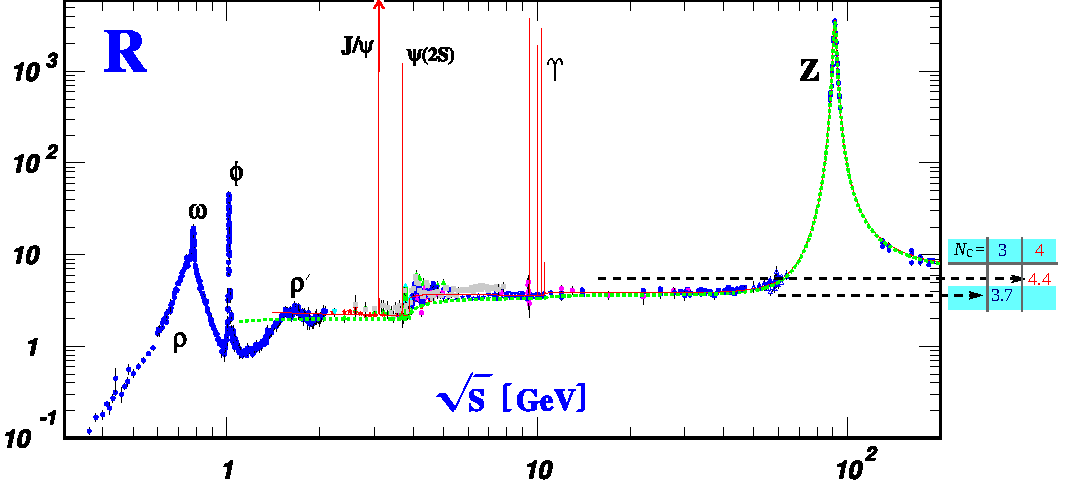
\includegraphics[scale=0.9]{r}
  \caption{Datos para $R$}
  \label{fig:r}
\end{figure}

Si queremos que el color sea una carga conservada como la carga el\'ectrica, o la de isosp\'\i n d\'ebil, esta debe ser la consecuencia de una simetr\'\i a gauge local. Para tener tres cargas diferentes la posibilidad m\'as simple es imponer la simetr\'\i a $SU(3)_c$, tal que tengamos un vector compuesto de 3 espinores de Dirac en el espacio de color:
\begin{equation}
  \Psi=
  \begin{pmatrix}
    \psi_r\\
    \psi_b\\
    \psi_g
  \end{pmatrix}
  =
  \begin{pmatrix}
    q_r\\
    q_b\\
    q_g
  \end{pmatrix}.
\end{equation}
El Lagrangiano de Dirac con invarianza gauge global $SU(3)$, para un quark, se puede escribir como
\begin{equation}
  \label{eq:128}
  \mathcal{L}_{\text{global}}=i\bar{\Psi}\gamma^\mu\partial_\mu\Psi-m\bar{\Psi}\Psi,
\end{equation}
donde
\begin{equation}
  \Psi\to \Psi'=\exp\left(i\theta_a\frac{\lambda^a}{2}\right)\Psi.
\end{equation}
$a=1,\ldots,8$, $\lambda_a/2$ son los ocho generadores de $SU(3)$ y $\theta_a$ son los par\'ametros de la transformaci\'on global. 

En un an\'alisis similar al de la secci\'on \ref{sec:invar-gauge-local-2} tenemos que la Acci\'on invariante gauge local bajo $SU(3)_c$, se obtiene de reemplazar la derivada normal por la derivada covariante (ver ec.~\eqref{eq:78})
\begin{equation}
  \label{eq:127}
  \mathcal{L}_{\text{local}}=i\bar{\Psi}\gamma^\mu\mathcal{D}_\mu\Psi-m\bar{\Psi}\Psi
  -\frac{1}{2}\operatorname{Tr}\left(\mathbf{G}^{\mu\nu}\mathbf{G}_{\mu\nu}\right),
\end{equation}
donde
\begin{align}
  \Psi\to \Psi'&=\exp\left[i\theta_a(x)\frac{\lambda^a}{2}\right]\Psi\nonumber\\
  \mathcal{D}_\mu\Psi\to \left(\mathcal{D}_\mu\Psi\right)'&
  =\exp\left[i\theta_a(x)\frac{\lambda^a}{2}\right]\mathcal{D}_\mu\Psi,
\end{align}
con
\begin{equation}
  \mathcal{D}_\mu=\partial_\mu-i g_s\frac{\lambda_a}{2}G_\mu^a\equiv\partial_\mu-i g_s {G}_\mu
\end{equation}
con la definici\'on de esta matriz $3\times3$ similar a la de la ec.~\eqref{eq:71}
\begin{equation}
  \left({G}_\mu\right)_{\alpha\beta}=\left(\frac{\lambda_a}{2}\right)_{\alpha\beta}G_\mu^a
\end{equation}
En t\'erminos, la transformaci\'on de los campos gauge esta dada por
\begin{equation}
    {G}^\mu\to\left({G}^\mu\right)'=U{G}^\mu U-\frac{i}{g_s}\left(\partial^\mu U\right)U^\dagger.
\end{equation}
Similarmente, definiendo la matriz $3\times3$, como se hizo en la ec.~\eqref{eq:126}
\begin{align}
  {G}^{\mu\nu}&=\frac{i}{g_s}[\mathcal{D}^\mu,\mathcal{D}^\nu]\equiv\frac{\lambda_a}{2}G^{\mu\nu}_a,
\end{align}
donde
\begin{equation}
  \label{eq:258}
  G^{\mu\nu}_a=\partial^\mu G^\nu_a-\partial^\nu G^\mu_a+g_s f^{abc}G^\mu_b G^\nu_c\equiv\widetilde{G}^{\mu\nu}_a+g_s f^{abc}G^\mu_b G^\nu_c,
\end{equation}
con
\begin{equation}
  \widetilde{G}^{\mu\nu}_a=\partial^\mu G^\nu_a-\partial^\nu G^\mu_a
\end{equation}

y $f^{abc}$ son las constantes de estructura fina de $SU(3)$
\begin{equation}
  \left[\frac{\lambda^a}{2},\frac{\lambda^b}{2}\right]=if^{abc}\frac{\lambda^c}{2}.
\end{equation}
Definiendo el producto vectorial de $SU(3)$ como
\begin{align}
  \left(\mathbf{A}\times\mathbf{B}\right)_a=f_{abc}A^b B^c\,,
\end{align}
si $\mathbf{G}^\mu$ es un vector en el espacio $SU(3)$ con las 8 componentes $G^\mu_a$, podemos escribir la ec.~\eqref{eq:258} como en la secci\'on \ref{sec:phi-como-un}
\begin{align}
  \mathbf{G}^{\mu\nu}=\partial^\mu \mathbf{G}^\nu-\partial^\nu \mathbf{G}^\mu+g_s \mathbf{G}^\mu\times \mathbf{G}^\nu\,,
\end{align}
donde $\mathbf{G}^{\mu\nu}$ es el vector en el espacio $SU(3)$ con las 8 componentes $G^{\mu\nu}_a$.
Expandiendo el Lagrangiano en ec.~(\ref{eq:127}), tenemos
\begin{align}
  \mathcal{L}=&i\bar{\Psi}\gamma^\mu\left(\partial_\mu-i g_s\frac{\lambda_a}{2}G_\mu^a\right)\Psi
  -m\bar{\Psi}\Psi- \frac{1}{4}G^{\mu\nu}_a G_{\mu\nu}^a\nonumber\\
=&i\bar{\Psi}\gamma^\mu\partial_\mu\Psi-m\bar{\Psi}\Psi+g_s\bar{\Psi}\gamma^\mu\frac{\lambda_a}{2}G_\mu^a\Psi
  - \frac{1}{4}G^{\mu\nu}_a G_{\mu\nu}^a\nonumber\\
=&i\bar{\Psi}\gamma^\mu\partial_\mu\Psi-m\bar{\Psi}\Psi+g_s\bar{\Psi}\gamma^\mu\frac{\lambda_a}{2}\Psi G_\mu^a
  - \frac{1}{4}\widetilde{G}^{\mu\nu}_a \widetilde{G}_{\mu\nu}^a\nonumber\\
  &- \frac{1}{4}\left(g_s\widetilde{G}^{\mu\nu}_af_{a d e}G^d_\mu G^e_\nu
    +g_sf^{a b c}G_b^\mu G_c^\nu\widetilde{G}_{\mu\nu}^a
    +g_s^2f^{a b c}f_{a d e}G_b^\mu G_c^\nu G^d_\mu G^e_\nu\right)
\end{align}
%\left(\right)
\begin{equation}
  \mathcal{L}=\mathcal{L}_{\text{global}}+\mathcal{L}_{\text{gauge}}+\mathcal{L}_{\text{SI}},
\end{equation}

donde
\begin{align}
\mathcal{L}_{\text{global}}=&i\bar{\Psi}\gamma^\mu\partial_\mu\Psi-m\bar{\Psi}\Psi\nonumber\\
  \mathcal{L}_{\text{gauge}}=&g_s\bar{\Psi}\gamma^\mu\frac{\lambda_a}{2}\Psi G_\mu^a
  - \frac{1}{4}\widetilde{G}^{\mu\nu}_a \widetilde{G}_{\mu\nu}^a\nonumber\\
=&-\frac{1}{4}\left(\partial^\mu G^\nu_a-\partial^\nu G^\mu_a\right)\left(\partial_\mu G_\nu^a-\partial_\nu G_\mu^a\right)+J^\nu_aG_\nu^a,
\end{align}
es la nueva corriente conservada de interacci\'on fuerte que surge como consecuencia de la invarianza gauge local $SU(3)$. 
\begin{align}
  \mathcal{L}_{\text{SI}}&=- \frac{1}{4}\left(g_s\widetilde{G}^{\mu\nu}_af_{a d e}G^d_\mu G^e_\nu
    +g_sf^{a b c}G_b^\mu G_c^\nu\widetilde{G}_{\mu\nu}^a
    +g_s^2f^{a b c}f_{a d e}G_b^\mu G_c^\nu G^d_\mu G^e_\nu\right)\nonumber\\
  &=- \frac{g_s}{2}f^{a b c}\widetilde{G}_{\mu\nu}^aG_b^\mu G_c^\nu
    +\frac{g_s^2}{4}f^{a b c}f_{a d e}G_b^\mu G_c^\nu G^d_\mu G^e_\nu\nonumber\\
  &=-\frac{g_s}{2}f^{abc}\left(\partial^\mu G^\nu_a-\partial^\nu G^\mu_a\right)G^b_\mu G^c_\nu-\frac{g_s^2}{4}f^{abc}f_{ade}G^\mu_bG^\nu_cG^d_\mu G^e_\nu,
\end{align}
son los t\'erminos de autointeraccci\'on gauge.

La coorriente de color
\begin{align}
j^\mu&\propto\frac{\partial\mathcal{L}}{\partial\left(\partial_\mu\Psi\right)}\delta\Psi+\delta\bar{\Psi}\frac{\partial\mathcal{L}}{\partial\left(\partial_\mu\bar{\Psi}\right)}
+\frac{\partial\mathcal{L}}{\partial\left(\partial_\mu G_\nu^a\right)}\delta G_\nu^a\nonumber\\
    \propto&i\bar{\Psi}\gamma^\mu i\theta^a(x)\frac{\lambda_a}{2}\Psi-G^{\mu\nu}_a\left(\frac{1}{g_s}\partial_\nu\theta^a+f_{abc}G_\nu^b\theta^c\right)\nonumber\\
   \propto&-\theta^a(x)\bar{\Psi}\gamma^\mu\frac{\lambda_a}{2}\Psi-\frac{1}{g_s}G^{\mu\nu}_a\partial_\nu\theta^a-G^{\mu\nu}_df_{dba}G_\nu^b\theta^a\nonumber\\
   \propto&-\theta^a(x)\bar{\Psi}\gamma^\mu\frac{\lambda_a}{2}\Psi-\left(\mathbf{G}^{\mu\nu}\times\mathbf{G}_\nu^b\right)_a\theta^a-\frac{1}{g_s}\partial_\nu(G^{\mu\nu}_a\theta^a)+
   \frac{1}{g_s}\theta^a\partial_\nu G^{\mu\nu}_a
\end{align}

Quitando el t\'ermino con derivada total
\begin{align}
\theta^aj^\mu_a \propto&-\theta^a(x)\left[\bar{\Psi}\gamma^\mu\frac{\lambda_a}{2}\Psi+\left(\mathbf{G}^{\mu\nu}\times\mathbf{G}_\nu^b\right)_a
-\frac{1}{g_s}\partial_\nu G^{\mu\nu}_a\right]
\end{align}
%\left(\right)
Eliminndo de nuevo el termino con derivada total, definimos
\begin{equation}
\label{eq:255}
j^\mu_a=-g_s\left[\bar{\Psi}\gamma^\mu\frac{\lambda_a}{2}\Psi+\left(\mathbf{G}^{\mu\nu}\times\mathbf{G}_\nu^b\right)_a\right]
\end{equation}


Todas las interacciones est\'an determinadas en t\'erminos de una \'unica constante de acoplamiento $g_s$. Las autointeracciones gauge pueden explicar aspectos de la interacci\'on fuerte como la libertada asint\'otica, que consiste en que las interacciones fuertes se vuelven m\'as d\'ebiles a distancias cortas. 

En t\'erminos de \'\i ndices de color la corriente, y las otras partes del Lagrangiano, pueden escribirse como
\begin{equation}
  \label{eq:223}
  J^\mu_a=-g_s\bar{q}^\alpha\gamma^\mu q^\beta\left(\frac{\lambda_a}{2}\right)_{\alpha\beta}.
\end{equation}
Note que tanto para la Electrodin\'amica Cu\'antica como para la Cromodin\'amica Cu\'antica la corriente $\bar{\psi}\Gamma\psi$ es vectorial. Para las interacciones d\'ebiles la estructura es m\'as complicada y requiere un conocimiento m\'as profundo de la ecuaci\'on de Dirac y sus soluciones.

\subsection{Ecuaciones de Euler--Lagrange}
\label{sec:ecuaciones-de-euler-1}
Sigiendo los mismos procedimientos anteriores debemos llegar a los siguientes resultados. Para el campo $\Psi$
\begin{align}
  (i\gamma^\mu\mathcal{D}_\mu-m)\Psi=0\,,
\end{align}
mientras que para los campos $\mathbf{G}^{\mu\nu}$
\begin{align}
  \mathcal{D}_\mu \mathbf{G}^{\mu\nu}=&\mathbf{J}^\nu\,,
\end{align}
donde el vector en espacio $SU(3)$ $\mathbf{J}^\nu$ tiene las 8 componentes $J^\nu_a$ dadas en la ec.~\eqref{eq:255}. Como $\mathbf{G}^{\mu\nu}$ es una matrix $8\times8$, la derivada covariante debe estar en la representaci\'on adjunta como en la ec.~\eqref{eq:256}. La ecuaci\'on~\eqref{eq:257} aplicada a $SU(3)$ es por consiguiente
\begin{align}
  \mathcal{D}_\mu \mathbf{G}^{\mu\nu}=&\partial_\mu\mathbf{G}^{\mu\nu}+g_s \mathbf{G}_\mu\times\mathbf{G}^{\mu\nu}\nonumber\\
  \mathcal{D}_\mu {G}^{\mu\nu}_a=&\partial_\mu{G}^{\mu\nu}_a+g_s f_{abc}{G}_\mu^b{G}^{\mu\nu}_c
\end{align}
%\left(\right)
\begin{align}
  \partial_\mu G^{\mu\nu}_a=-g_s\left[f_{abc}G^b_\mu G^{\mu\nu}_c+\bar{\Psi}\gamma^\nu\frac{\lambda_a}{2}\Psi  \right]
\end{align}
donde
\begin{align}
  j^\nu_a=&-g_s\left[f_{abc}G^b_\mu G^{\mu\nu}_c+\bar{\Psi}\gamma^\nu\frac{\lambda_a}{2}\Psi  \right]\nonumber\\
=&-g_s\left[-\left(\mathbf{G}^{\mu\nu}\times\mathbf{G}_\nu^b\right)_a+\bar{\Psi}\gamma^\nu\frac{\lambda_a}{2}\Psi  \right]\nonumber\\
\end{align}
Como $\mathbf{G}^{\mu\nu}=-\mathbf{G}^{\nu\mu}$ se sigue que
\begin{equation}
  \partial_\nu j^\nu_a=0
\end{equation}
y tenemos las ocho corrientes conservadas.


%\left(\right)
%%% Local Variables: 
%%% mode: latex
%%% TeX-master: "fullnotes"
%%% End: 
